\section{Results}

% We show images from the UF9 and DTLZ4 functions due to space limitations, but similar images for the other problems are available in the supplementary materials.

% Ideias para resultados
%%% In terms of IGD and HV, we can seee that in general, using resource allocation performs better than not using resource allocation. RI and Norm achieve similar results, and Random as well for HV, (but not IGD). These results are indicated by the boxplot, the tables, the pareto front, and the willcoxon pairwise analysis. For the Moon Landing problem, all strategies found similar Hypervolume results.

%%% The fact that random performed as well as Norm and RI in HV indicates that there is still space for finding more appropriate priority functions?

%%% Figure 4 shows how the different strategies are allocating results for functions UF9 and DTLZ4. It is interesting to observe that RI and Norm assign similar priorities to the same subproblems in the DTLZ4. But they find opposite priorities to subproblems on the UF9 function.

%%% Dominance and feasibility
% Another difference that we see among the Resource Allocation strategies is found in the proportion of non dominated and feasible solutions. For the Benchmark problems, the Norm Strategy achieved a very high fraction of non-dominated solutions in the final solution set. In the Lunar Landing problem, the Norm strategy achieved a higher proportion of feasible solutions than the other resource allocation strategies.





\begin{table*}[!t]
	\begin{tabular}{llllll}
		\cline{6-6}
		\hline
		\rowcolor[gray]{.7} \multicolumn{1}{|l|}{\textbf{HV}}         & \multicolumn{1}{l|}{None} & \multicolumn{1}{l|}{MRDL} & \multicolumn{1}{l|}{Norm} & \multicolumn{1}{l|}{R.I.} & \multicolumn{1}{l|}{Random} \\ \hline \hline  \hline
		\multicolumn{1}{l}{Lunar}           & \multicolumn{1}{l}{0.656 (0.034)} & \multicolumn{1}{l}{\textbf{0.687 (0.057)}} & \multicolumn{1}{l}{0.666 (0.060)} & 0.683 (0.067)             &\multicolumn{1}{l} {0.664 (0.047)} \\ \hline \hline \hline
		\rowcolor[gray]{.95} \multicolumn{1}{l}{UF1}              & \multicolumn{1}{l}{0.861 (0.011)} & \multicolumn{1}{l}{0.863 (0.015)} & \multicolumn{1}{l}{0.833 (0.022)} & \textbf{0.88 (0.013)}             &\multicolumn{1}{l} {0.874 (0.015)} \\ %\hline \hline
		\multicolumn{1}{l}{UF2}              & \multicolumn{1}{l}{0.750 (0.009)} & \multicolumn{1}{l}{0.750 (0.005)} & \multicolumn{1}{l}{ 0.762 (0.010)} & 0.82 (0.008)             &\multicolumn{1}{l} {\textbf{0.83 (0.008)}} \\ %\hline \hline
		\rowcolor[gray]{.95}\multicolumn{1}{l}{UF3}              & \multicolumn{1}{l}{0.844 (0.044)} & \multicolumn{1}{l}{0.860 (0.043)} & \multicolumn{1}{l}{ \textbf{0.944 (0.018)}} & 0.918 (0.029)             &\multicolumn{1}{l}  {0.909 (0.037)} \\ %\hline \hline
		\multicolumn{1}{l}{UF4}              & \multicolumn{1}{l}{0.364 (0.005)} & \multicolumn{1}{l}{0.366 (0.003)} & \multicolumn{1}{l}{ 0.372 (0.003)} & 0.371 (0.004)             &\multicolumn{1}{l} {\textbf{0.373 (0.004)}} \\ %\hline \hline
		\rowcolor[gray]{.95}\multicolumn{1}{l}{UF5}              & \multicolumn{1}{l}{0.629 (0.022)} & \multicolumn{1}{l}{0.663 (0.024)} & \multicolumn{1}{l}{ 0.754 (0.034)} & \textbf{0.811 (0.015)}             &\multicolumn{1}{l} {0.810 (0.016)} \\ %\hline \hline
		\multicolumn{1}{l}{UF6}              & \multicolumn{1}{l}{0.661 (0.020)} & \multicolumn{1}{l}{0.660 (0.014)} & \multicolumn{1}{l}{ 0.662 (0.020)} & 0.686 (0.014)             &\multicolumn{1}{l} {\textbf{0.689 (0.015)}} \\ %\hline \hline
		\rowcolor[gray]{.95}\multicolumn{1}{l}{UF7}              & \multicolumn{1}{l}{0.803 (0.010)} & \multicolumn{1}{l}{0.801 (0.010)} & \multicolumn{1}{l}{ 0.818 (0.012)} & \textbf{0.837 (0.005)}             &\multicolumn{1}{l} {0.834 (0.006)} \\ %\hline \hline
		\multicolumn{1}{l}{UF8}              & \multicolumn{1}{l}{0.894 (0.004)} & \multicolumn{1}{l}{0.900 (0.004)} & \multicolumn{1}{l}{ 0.914 (0.005)} & \textbf{0.922 (0.003)}             &\multicolumn{1}{l} {0.916 (0.004)} \\ %\hline \hline
		\rowcolor[gray]{.95}\multicolumn{1}{l}{UF9}              & \multicolumn{1}{l}{0.931 (0.004)} & \multicolumn{1}{l}{0.932 (0.004)} & \multicolumn{1}{l}{ \textbf{0.944 (0.014)}} & 0.932 (0.004)             &\multicolumn{1}{l} {0.940 (0.008)} \\ %\hline \hline
		\multicolumn{1}{l}{UF10}              & \multicolumn{1}{l}{0860 (0.017)} & \multicolumn{1}{l}{0.786 (0.017)} & \multicolumn{1}{l}{ 0.835 (0.035)} & \textbf{0.861 (0.033)}             &\multicolumn{1}{l} {0.839 (0.026)} \\ \hline  \hline \hline
		\rowcolor[gray]{.95}\multicolumn{1}{l}{DTLZ1}              & \multicolumn{1}{l}{0.989 (0.003)} & \multicolumn{1}{l}{0.991 (0.004)} & \multicolumn{1}{l}{ 0.997 (0.002)} & 0.998 (0.002)             & \multicolumn{1}{l} {\textbf{0.998 (0.001)}} \\ %\hline \hline
		\multicolumn{1}{l}{DTLZ2}              & \multicolumn{1}{l}{0.910 (0.002)} & \multicolumn{1}{l}{0.912 (0.002)} & \multicolumn{1}{l}{ \textbf{0.922 (0.001)}} & 0.921 (0.001)             & \multicolumn{1}{l} {\textbf{0.922 (0.001)}} \\ %\hline  \hline
		\rowcolor[gray]{.95}\multicolumn{1}{l}{DTLZ3}              & \multicolumn{1}{l}{0.960 (0.015)} & \multicolumn{1}{l}{0.969 (0.016)} & \multicolumn{1}{l}{ 0.992 (0.009)} &0.991 (0.009)             & \multicolumn{1}{l} {\textbf{0.993 (0.006)}} \\ %\hline \hline
		\multicolumn{1}{l}{DTLZ4}              & \multicolumn{1}{l}{0.905 (0.003)} & \multicolumn{1}{l}{0.907 (0.004)} & \multicolumn{1}{l}{0.920 (0.001)} &  \textbf{0.921 (0.004) }            & \multicolumn{1}{l} {0.918 (0.002)} \\ %\hline  \hline
		\rowcolor[gray]{.95}\multicolumn{1}{l}{DTLZ5}              & \multicolumn{1}{l}{0.895 (0.003)} & \multicolumn{1}{l}{0.898 (0.002)} & \multicolumn{1}{l}{ \textbf{0.910 (0.001)} }&0.908 (0.002)             & \multicolumn{1}{l} {\textbf{0.910 (0.001)}} \\ %\hline \hline
		\multicolumn{1}{l}{DTLZ6}              & \multicolumn{1}{l}{0.837 (0.035)} & \multicolumn{1}{l}{0.860 (0.021)} & \multicolumn{1}{l}{ \textbf{0.999 ($>$0.000)}} & 0.999 (0.001)             & \multicolumn{1}{l} {0.999 (0.001)} \\ %\hline  \hline
		\rowcolor[gray]{.95}\multicolumn{1}{l}{DTLZ7}              & \multicolumn{1}{l}{0.325 (0.056)} & \multicolumn{1}{l}{0.339 (0.048)} & \multicolumn{1}{l}{ \textbf{0.688 (0.005)}} &0.688 (0.006)             & \multicolumn{1}{l} {0.660 (0.011)} \\ %\hline
		\hline \hline  \hline
		%	\end{tabular}
		%	\caption{HV median and standard deviation, in parenthesis. The best values found by a priority function is in bold. None (the MOEA/D-DE with no priority function).}
		%	\label{table_hv}
		%\end{table*}
		%
		%\begin{table*}[!t]
		%	\begin{tabular}{llllll}
		\cline{6-6}
		\hline
		\rowcolor[gray]{.7} \multicolumn{1}{|l|}{\textbf{IGD}}         & \multicolumn{1}{l|}{None} & \multicolumn{1}{l|}{MRDL} & \multicolumn{1}{l|}{Norm} & \multicolumn{1}{l|}{R.I.} & \multicolumn{1}{l|}{Random} \\ \hline \hline  \hline
		UF1              & 0.140 (0.013) & 0.128 (0.015) & 0.109 (0.016) & 0.090 (0.012)             & 0.093 (0.014) \\ %\hline \hline
		\rowcolor[gray]{.95}UF2              & 0.082 (0.006) & 0.080 (0.007) & 0.060 (0.005) & 0.060 (0.005)             & \textbf{0.060 (0.004)} \\ %\hline \hline
		UF3              & \multicolumn{1}{l}{0.260 (0.012)} & \multicolumn{1}{l}{0.257 (0.009)}
		& \multicolumn{1}{l}{ \textbf{0.168 (0.025)}} & 0.183 (0.335)             &  \multicolumn{1}{l} {0.214 (0.030)} \\ %\hline \hline
		\rowcolor[gray]{.95}UF4              & \multicolumn{1}{l}{0.100 (0.003)} & \multicolumn{1}{l}{ 0.100 (0.023)} & \multicolumn{1}{l}{ \textbf{0.095 (0.002)}} & 0.095 (0.003)             & \multicolumn{1}{l} {\textbf{0.095 (0.002)}} \\ %\hline \hline
		UF5              & \multicolumn{1}{l}{1.759 (0.080)} & \multicolumn{1}{l}{1.648 (0.091)} & \multicolumn{1}{l}{ \textbf{0.972 (0.056)}} & 1.056 (0.064)            & \multicolumn{1}{l} {1.085 (0.073)} \\% \hline \hline
		\rowcolor[gray]{.95}UF6              & \multicolumn{1}{l}{0.121 (0.027)} & \multicolumn{1}{l}{0.120 (0.017)} & \multicolumn{1}{l}{ 0.100 (0.016)} & \textbf{0.078 (0.014)}            & \multicolumn{1}{l} {0.079 (0.016)} \\ %\hline		 \hline
		UF7               & \multicolumn{1}{l}{0.125 (0.018)} & \multicolumn{1}{l}{0.127 (0.015)} & \multicolumn{1}{l}{ \textbf{0.061 (0.006)}} & 0.068 (0.005)             & \multicolumn{1}{l} {0.074 (0.005)} \\ %\hline \hline
		\rowcolor[gray]{.95}UF8              & \multicolumn{1}{l}{0.286 (0.012)} & \multicolumn{1}{l}{0.279 (0.010)} & \multicolumn{1}{l}{ \textbf{0.229 (0.014)}} & 0.257 (0.020)             & \multicolumn{1}{l} {0.232 (0.006)} \\ %\hline \hline
		UF9               & \multicolumn{1}{l}{0.451 (0.012)} & \multicolumn{1}{l}{0.439 (0.015)} & \multicolumn{1}{l}{ \textbf{0.385 (0.020)}} & 0.420 (0.017)             & \multicolumn{1}{l} {0.400 (0.018)} \\ %\hline \hline
		\rowcolor[gray]{.95}UF10              & \multicolumn{1}{l}{3.693 (0.200)} & \multicolumn{1}{l}{3.456 (0.229)} & \multicolumn{1}{l}{ 2.380 (0.241)} & \textbf{2.364 (0.272)}             & \multicolumn{1}{l} {2.639 (0.253)} \\ \hline  \hline  \hline
		DTLZ1               & \multicolumn{1}{l}{381.5 (125.1)} & \multicolumn{1}{l}{337.5 (164.9)} & \multicolumn{1}{l}{231.0 (086.4)} & 222.5 (105.7)             & \multicolumn{1}{l} {\textbf{205.8 (093.8)}} \\ %\hline \hline
		\rowcolor[gray]{.95}DTLZ2           & \multicolumn{1}{l}{0.158 (0.013)} & \multicolumn{1}{l}{0.143 (0.010)} & \multicolumn{1}{l}{ \textbf{0.072 (0.007)}} & 0.095 (0.013)             & \multicolumn{1}{l} {0.085 (0.010)} \\ %\hline  \hline
		DTLZ3              & \multicolumn{1}{l}{1248 (300.2)} & \multicolumn{1}{l}{1047 (405.6)} & \multicolumn{1}{l}{572.2 (312.9)} & \textbf{495.2 (267.6)}            & \multicolumn{1}{l} {557.2 (234.3)} \\ %\hline \hline
		\rowcolor[gray]{.95}DTLZ4              & \multicolumn{1}{l}{0.173 (0.024)} & \multicolumn{1}{l}{0.165 (0.037)} & \multicolumn{1}{l}{0.076 (0.007)} & \textbf{0.072 (0.08)}             & \multicolumn{1}{l} {0.093 (0.017)} \\ %\hline  \hline
		DTLZ5              & \multicolumn{1}{l}{0.152 (0.015)} & \multicolumn{1}{l}{0.139 (0.010)} & \multicolumn{1}{l}{\textbf{0.076 (0.007)}} & 0.084 (0.010)            & \multicolumn{1}{l} {0.080 (0.008)} \\ %\hline \hline
		\rowcolor[gray]{.95}DTLZ6             & \multicolumn{1}{l}{15.97 (2.148)} & \multicolumn{1}{l}{14.89 (1.347)} & \multicolumn{1}{l}{\textbf{0.007 (0.001)}} & 0.508 (0.423)            & \multicolumn{1}{l} {0.664 (0.585)} \\ %\hline   \hline
		DTLZ7             & \multicolumn{1}{l}{1.033 (0.153)} & \multicolumn{1}{l}{1.012 (0.130)} & \multicolumn{1}{l}{0.044 (0.010)} & \textbf{0.042 (0.013)}            & \multicolumn{1}{l} {0.105 (0.029)} \\ %\hline
		
	\end{tabular}
	\caption{HV and IGD medians and standard deviations, in parenthesis for every function/priority function. The best values found by a priority function are in bold. Standard deviation was used as tie breaker.\\
	}
	\label{table_hv_igd}
\end{table*}

\begin{table*}[!t]
	\begin{tabular}{llllll}
		\cline{6-6}
		\hline
		\rowcolor[gray]{.7} \multicolumn{1}{|l|}{\textbf{Proportion}}         & \multicolumn{1}{l|}{None} & \multicolumn{1}{l|}{MRDL} & \multicolumn{1}{l|}{Norm} & \multicolumn{1}{l|}{R.I.} & \multicolumn{1}{l|}{Random} \\ \hline \hline  \hline
		
		Lunar (Feasible (\%))           & 0.1291 (0.08) & 0.0745 (0.13) & 0.1113 (0.16) & 0.0929 (0.19)             & 0.0550 (0.10) \\
		
		\rowcolor[gray]{.95}Lunar (Non-dominated (\%))           & 0.0016 (0.01) &0.0018 (0.01) & 0.0059 (0.09) & 0.0083 (0.09)             & 0.0030 (0.02) \\%\hline  \hline \hline
		
		UF (Non-dominated (\%))              & 0.34 (0.04) & 0.35 (0.04) & 0.84 (0.06) & 0.58 (0.10)             & 0.69 (0.05) \\ %\hline \hline \hline
		
		\rowcolor[gray]{.95}DTLZ (Non-dominated (\%))              & 0.10 (0.03) & 0.13 (0.03) & 0.97 (0.05) & 0.68 (0.19)             &  0.66 (0.13) \\ %\hline
		
	\end{tabular}
	\caption{Mean of the percentage of the median values and mean of the median values of the standard deviation (in parenthesis) of non-dominated solutions on UF and DTLZ benchmarks.\\
	}
	\label{minor_results}
\end{table*}

\begin{table}[!t]
	\begin{tabular}{lllll}
		\hline
		\rowcolor[gray]{.7} \multicolumn{1}{|l|}{\textbf{HV}}  & \multicolumn{1}{|l|}{MRDL} & \multicolumn{1}{l|}{None} & \multicolumn{1}{l|}{Norm} & \multicolumn{1}{l|}{R.I.} \\ \hline \hline \hline
		None                      & 0.82                      & -                         & -                         & -                         \\
		\rowcolor[gray]{.95}Norm                      & 2.9e-06                   & 6.2e-07                   & -                         & -                         \\
		R.I.                      & 8.6e-08                   & 1.3e-08                   & 0.82                      & -                         \\
		\rowcolor[gray]{.95}Random                    & 2.5e-06                   & 3.8e-07                   & 0.82                      & 0.82                      \\ \hline \hline \hline
		\rowcolor[gray]{.7} \multicolumn{1}{|l|}{\textbf{IGD}} & \multicolumn{1}{|l|}{MRDL} & \multicolumn{1}{l|}{None} & \multicolumn{1}{l|}{Norm} & \multicolumn{1}{l|}{R.I.} \\ \hline \hline \hline
		None                      & 0.478                     & -                         & -                         & -                         \\
		\rowcolor[gray]{.95}Norm                      & \textless 2e-16           & \textless 2.e-16          & -                         & -                         \\
		R.I.                      & 1.6e-13                   & 7.6e-14                   & 0.109                     & -                         \\
		\rowcolor[gray]{.95}Random                    & 7.7e-12                   & 5.0e-12                   & 0.002                     & 0.337
	\end{tabular}
	\caption{Statistical Analysis of the HV and IGD results based on the Pairwise Wilcoxon Rank Sum Test. No significant difference between MRDL and None, while the other three priority functions are statistically different from None.\\
	}
	\label{statistics}
\end{table}



%\begin{table}[!t]
%	\begin{tabular}{lllll}
%		\hline
%		\rowcolor[gray]{.7} \multicolumn{1}{|l|}{HV}  & \multicolumn{1}{|l|}{MRDL} & \multicolumn{1}{l|}{None} & \multicolumn{1}{l|}{Norm} & \multicolumn{1}{l|}{R.I.} \\ \hline \hline \hline
%		None                      & 0.82                      & -                         & -                         & -                         \\
%		\rowcolor[gray]{.95}Norm                      & 2.9e-06                   & 6.2e-07                   & -                         & -                         \\
%		R.I.                      & 8.6e-08                   & 1.3e-08                   & 0.82                      & -                         \\
%		\rowcolor[gray]{.95}Random                    & 2.5e-06                   & 3.8e-07                   & 0.82                      & 0.82                      \\ \hline \hline \hline
%		\rowcolor[gray]{.7} \multicolumn{1}{|l|}{IGD} & \multicolumn{1}{|l|}{MRDL} & \multicolumn{1}{l|}{None} & \multicolumn{1}{l|}{Norm} & \multicolumn{1}{l|}{R.I.} \\ \hline \hline \hline
%		None                      & 0.478                     & -                         & -                         & -                         \\
%		\rowcolor[gray]{.95}Norm                      & \textless 2e-16           & \textless 2.e-16          & -                         & -                         \\
%		R.I.                      & 1.6e-13                   & 7.6e-14                   & 0.109                     & -                         \\
%		\rowcolor[gray]{.95}Random                    & 7.7e-12                   & 5.0e-12                   & 0.002                     & 0.337 \hline \hline \hline
%%		\rowcolor[gray]{.7} \multicolumn{1}{|l|}{HV - Lunar Landing}  & \multicolumn{1}{|l|}{MRDL} & \multicolumn{1}{l|}{None} & \multicolumn{1}{l|}{Norm} & \multicolumn{1}{l|}{R.I.} \\ \hline \hline \hline
%%		None                      & 0.011                      & -                         & -                         & -                         \\
%%		\rowcolor[gray]{.95}Norm                      & 0.489                   & 0.848                   & -                         & -                         \\
%%		R.I.                      & 0.889                   & 0.598                   & 0.921                      & -                         \\
%%		\rowcolor[gray]{.95}Random                    & 0.517                   & 0.741                   & 0.921                      & 0.921                      \\ \hline \hline \hline
%	\end{tabular}
%	\caption{Statistical Analysis of the HV and IGD results based on the Pairwise Wilcoxon Rank Sum Test. This table shows that no significant difference was found between MRDL and None, although the other priority functions are statistically different to None. In the HV case, there is no significant difference between Norm, R.I., and Random. In the IGD case there is no significant difference between R.I. and Random, but there is between Norm and Random.
%	\label{statistics}
%\end{table}


\begin{figure*}[!t]
	%	\Large{Average performance on different tournament size - Gallagher's Gaussian 21-hi Peaks Function}
	\begin{subfigure}[b]{0.33\textwidth}
		\centering
	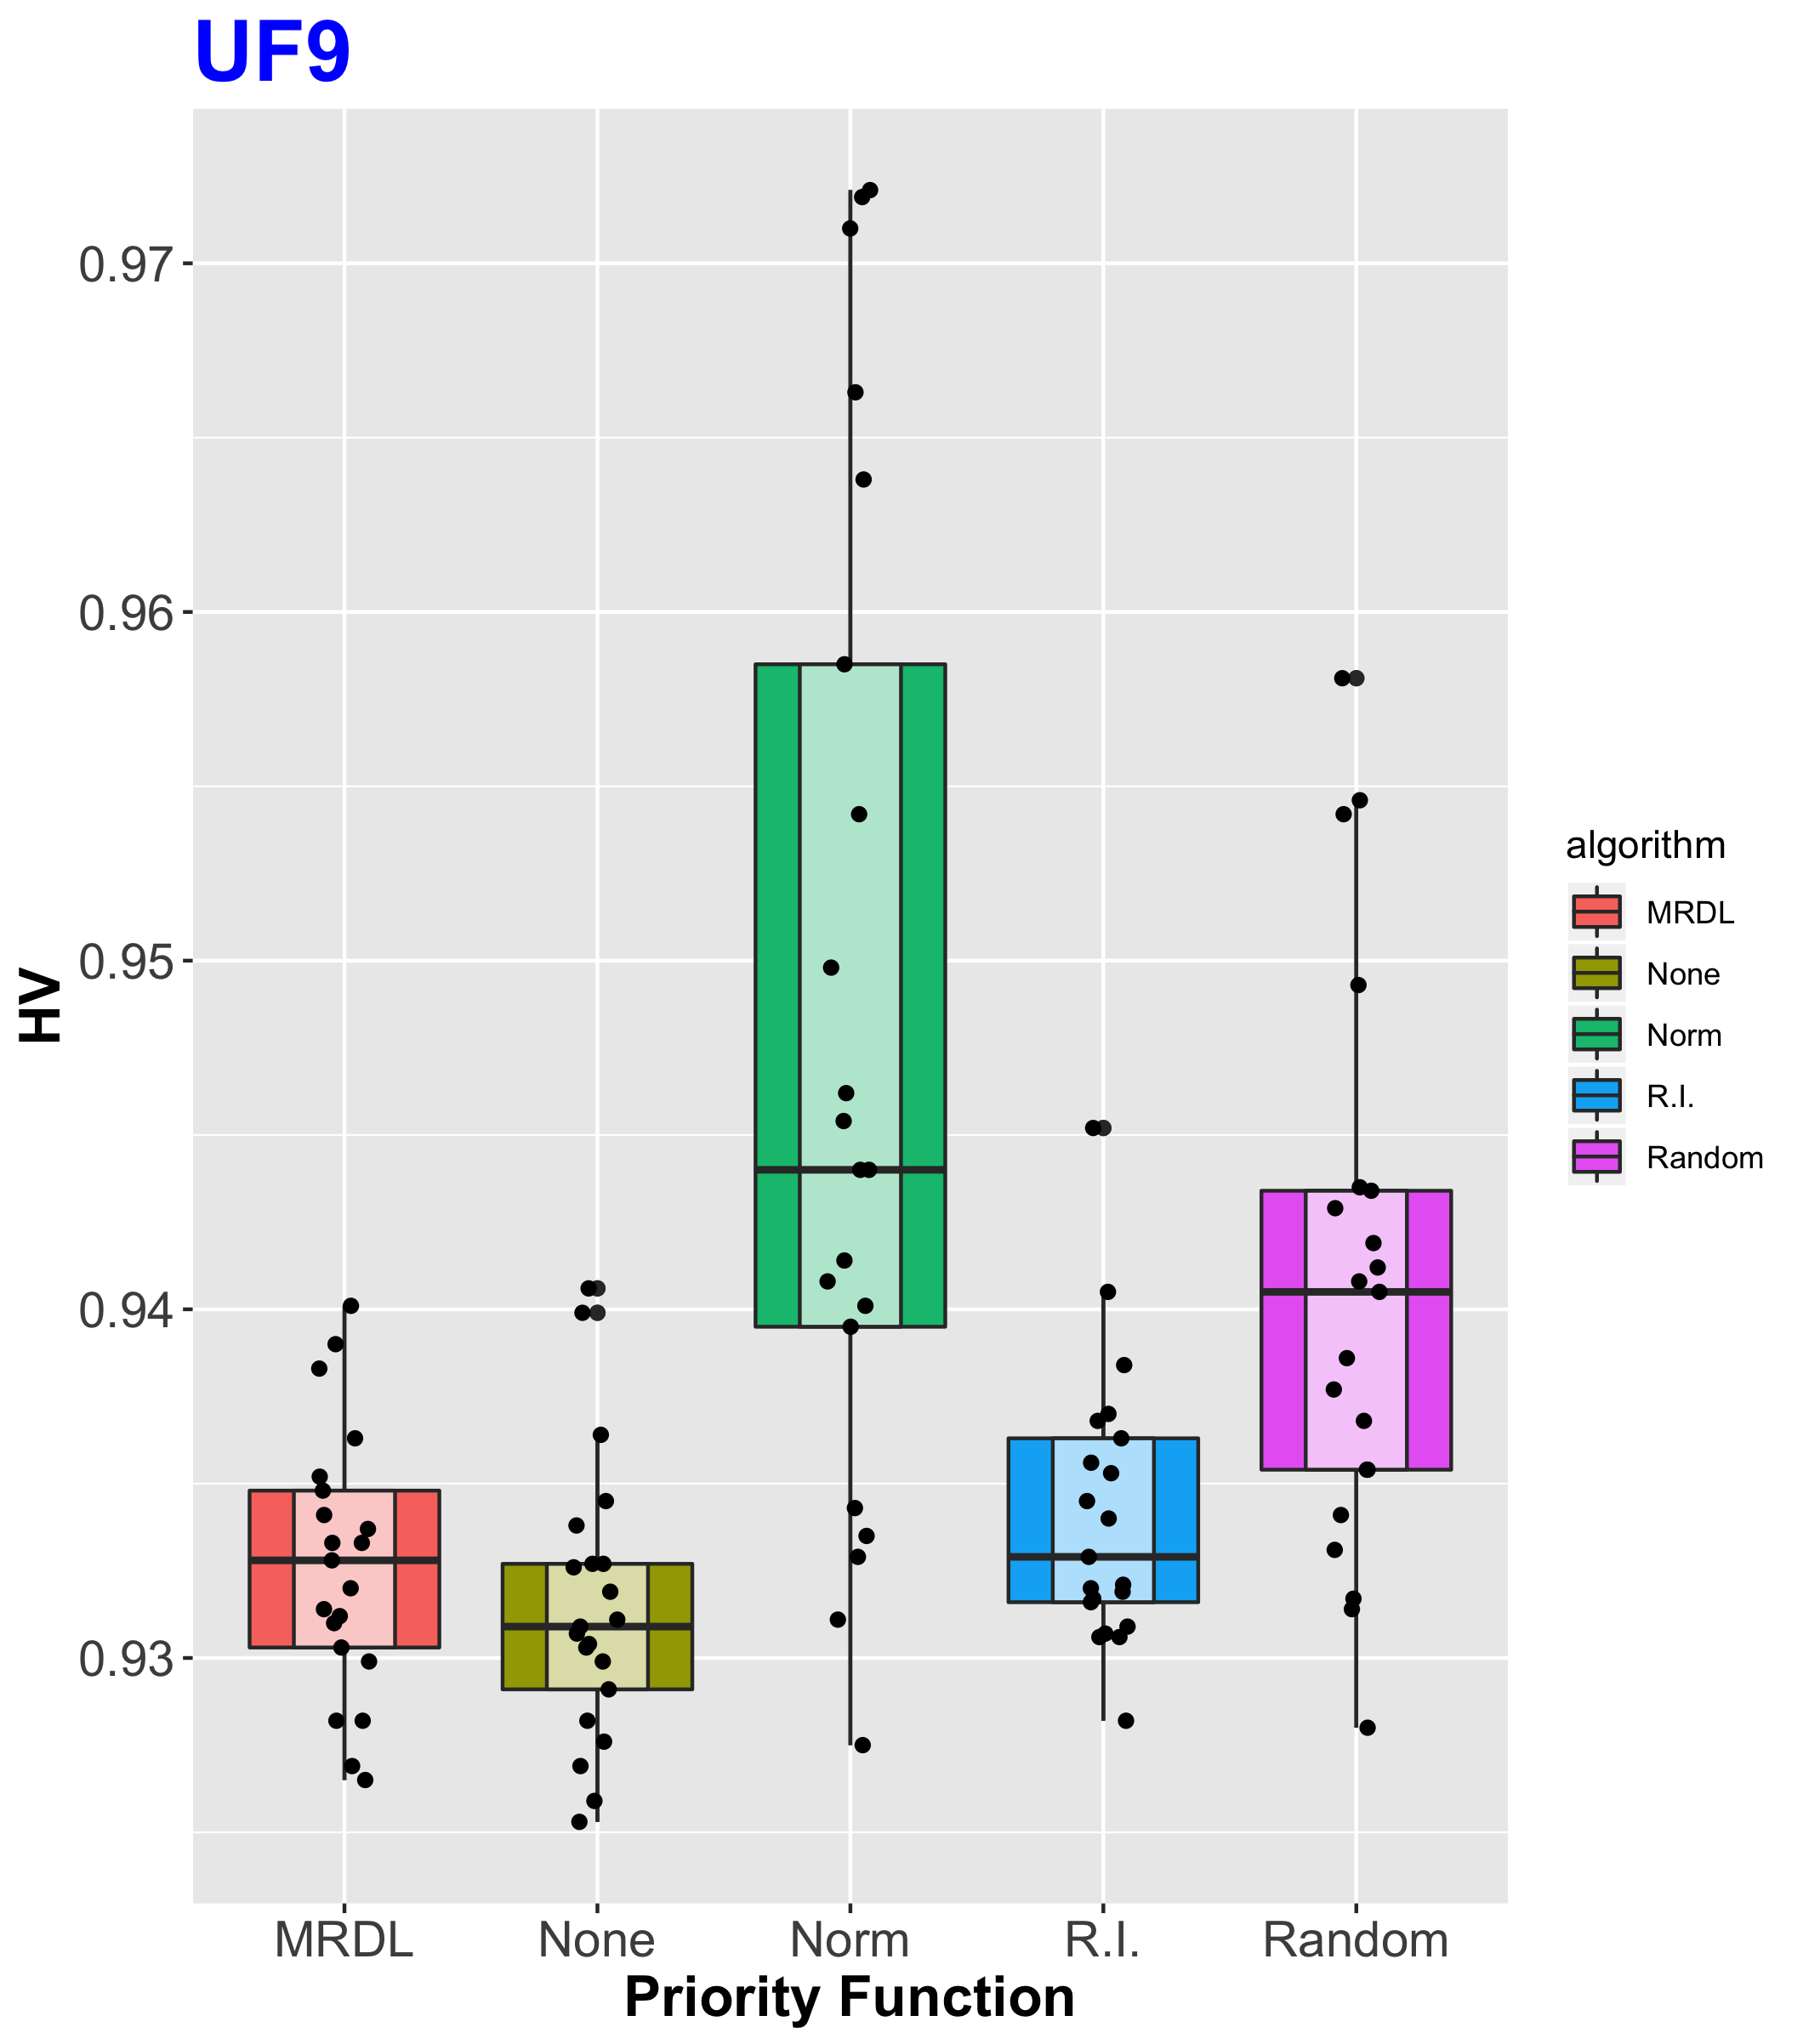
\includegraphics[width=1\textwidth, height=1\textwidth]{images/UF9_HV.png}
%	\caption{HV - UF3}
	\end{subfigure}
	\begin{subfigure}[b]{0.33\textwidth}
		\centering
	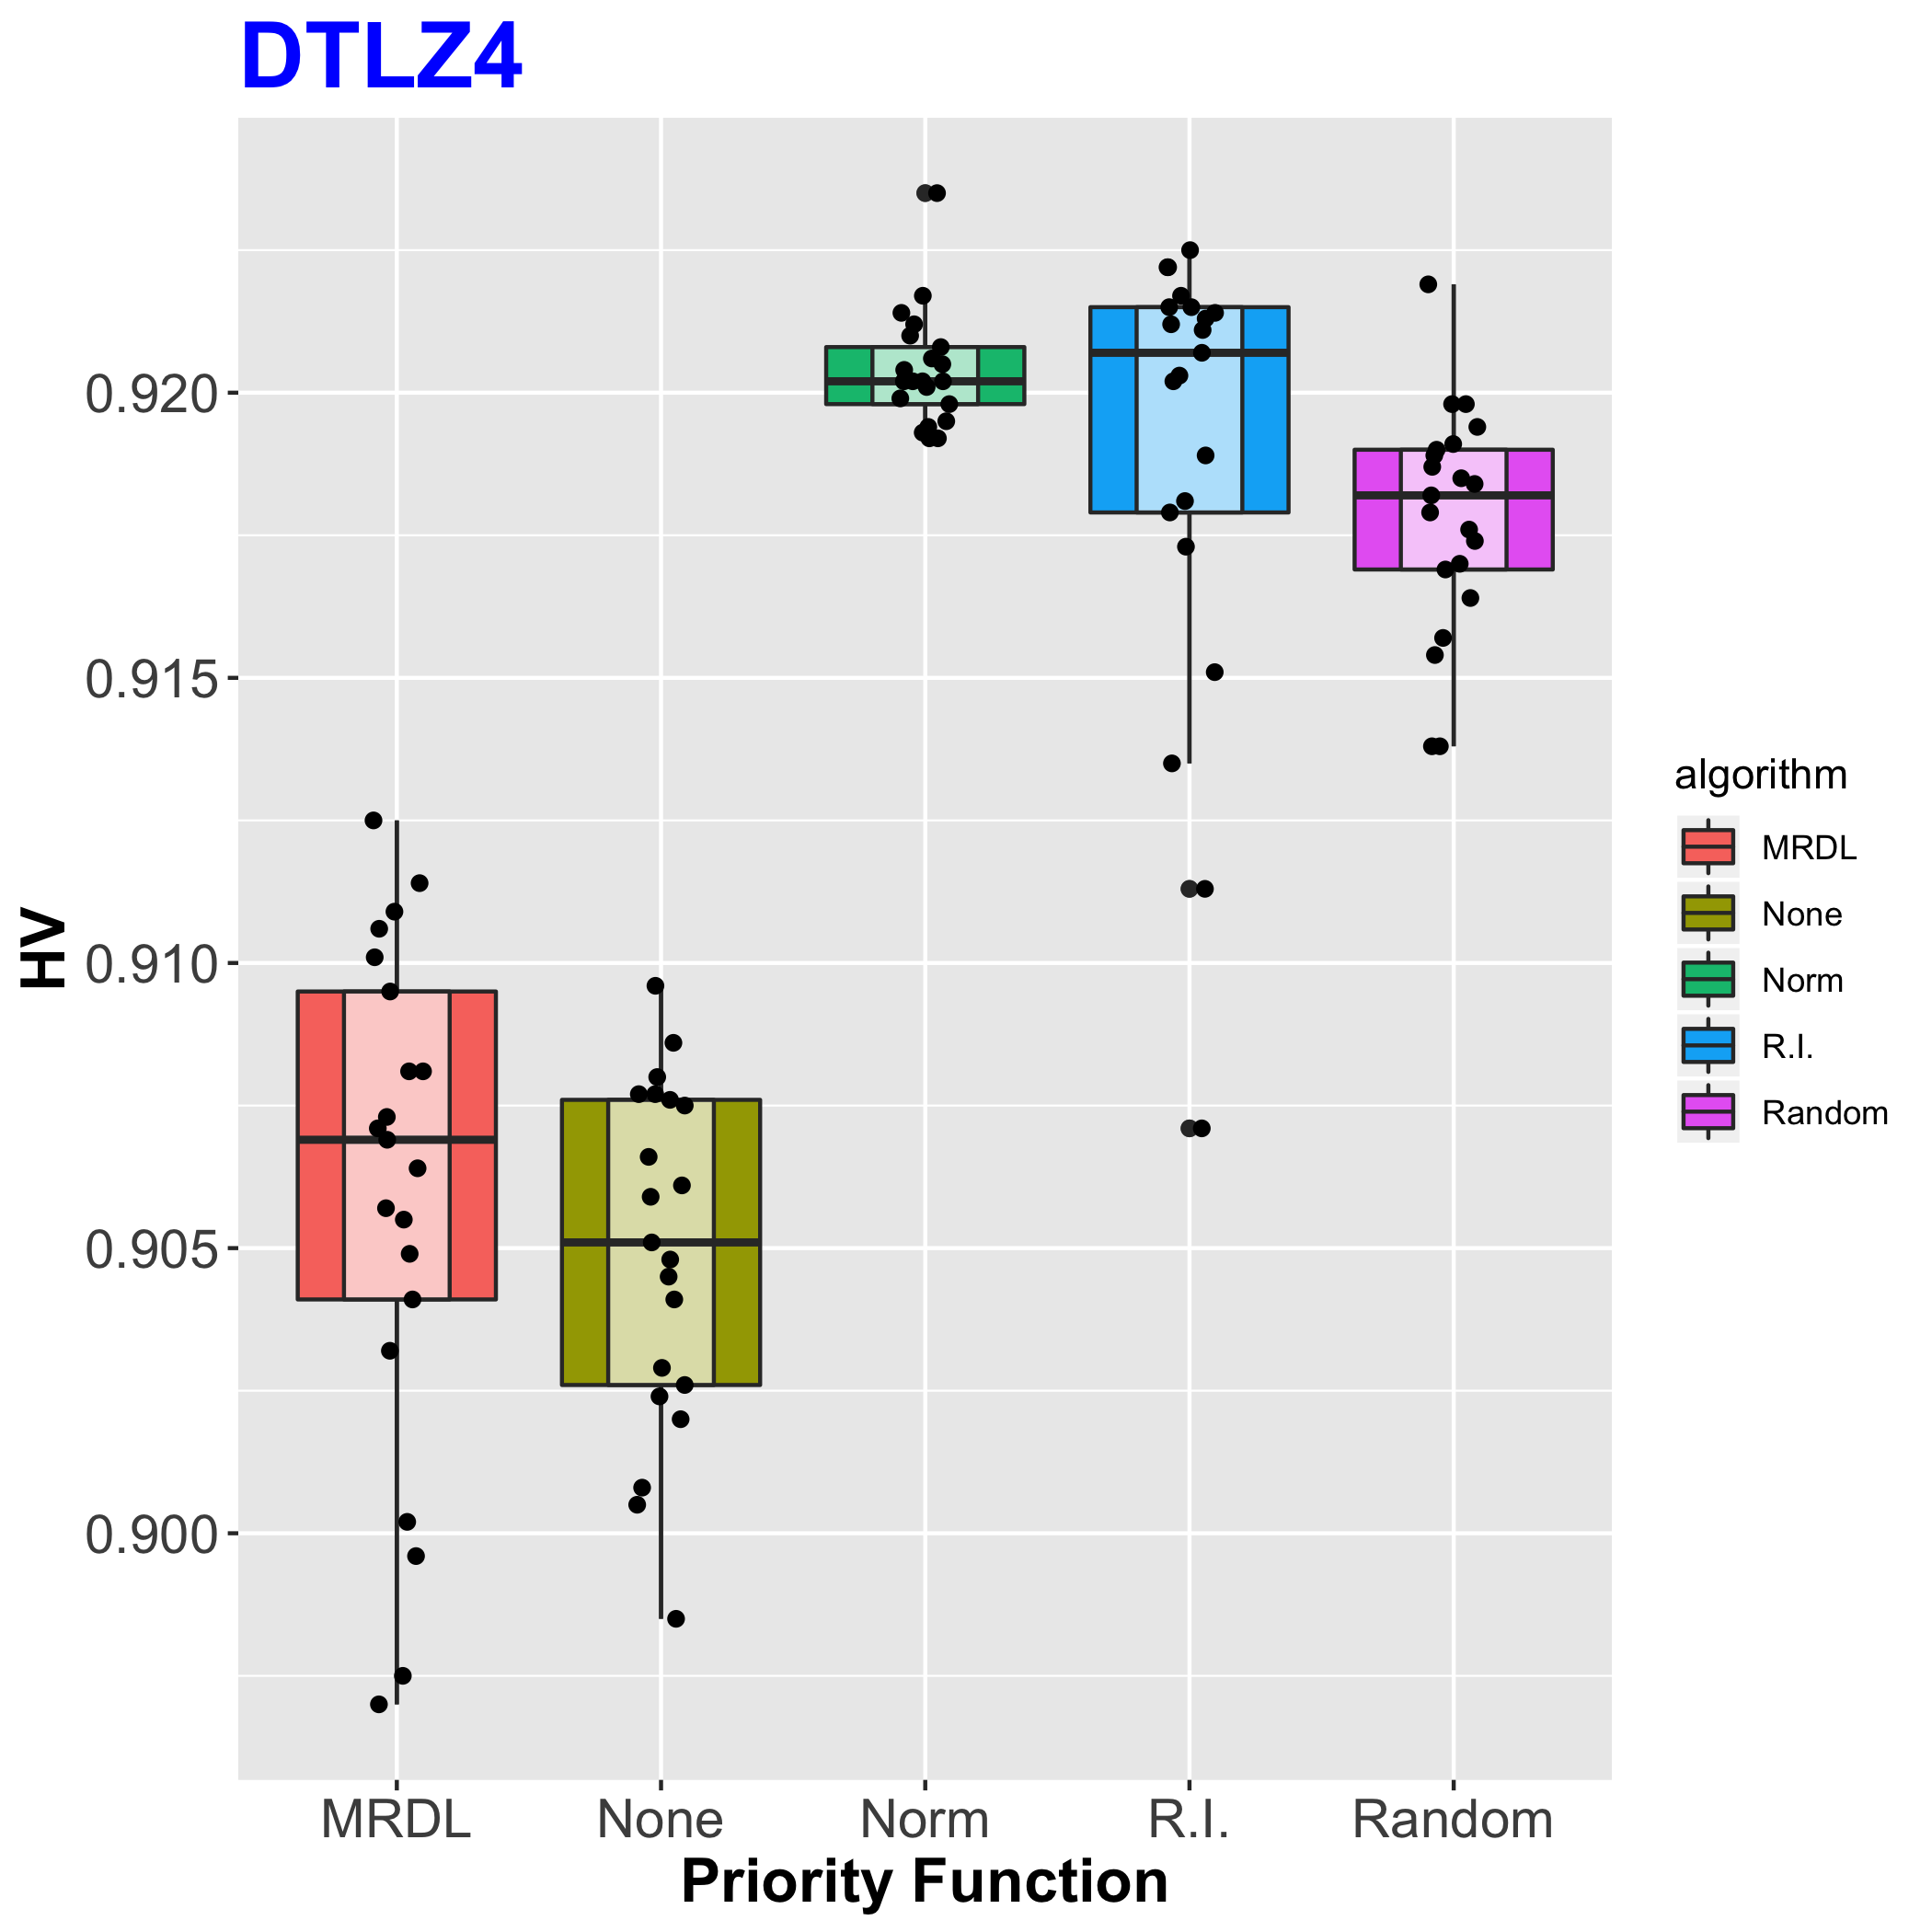
\includegraphics[width=1\textwidth, height=1\textwidth]{images/DTLZ4_HV.png}
%	\caption{HV - UF8}
	\end{subfigure}
\begin{subfigure}[b]{0.33\textwidth}
	\centering
	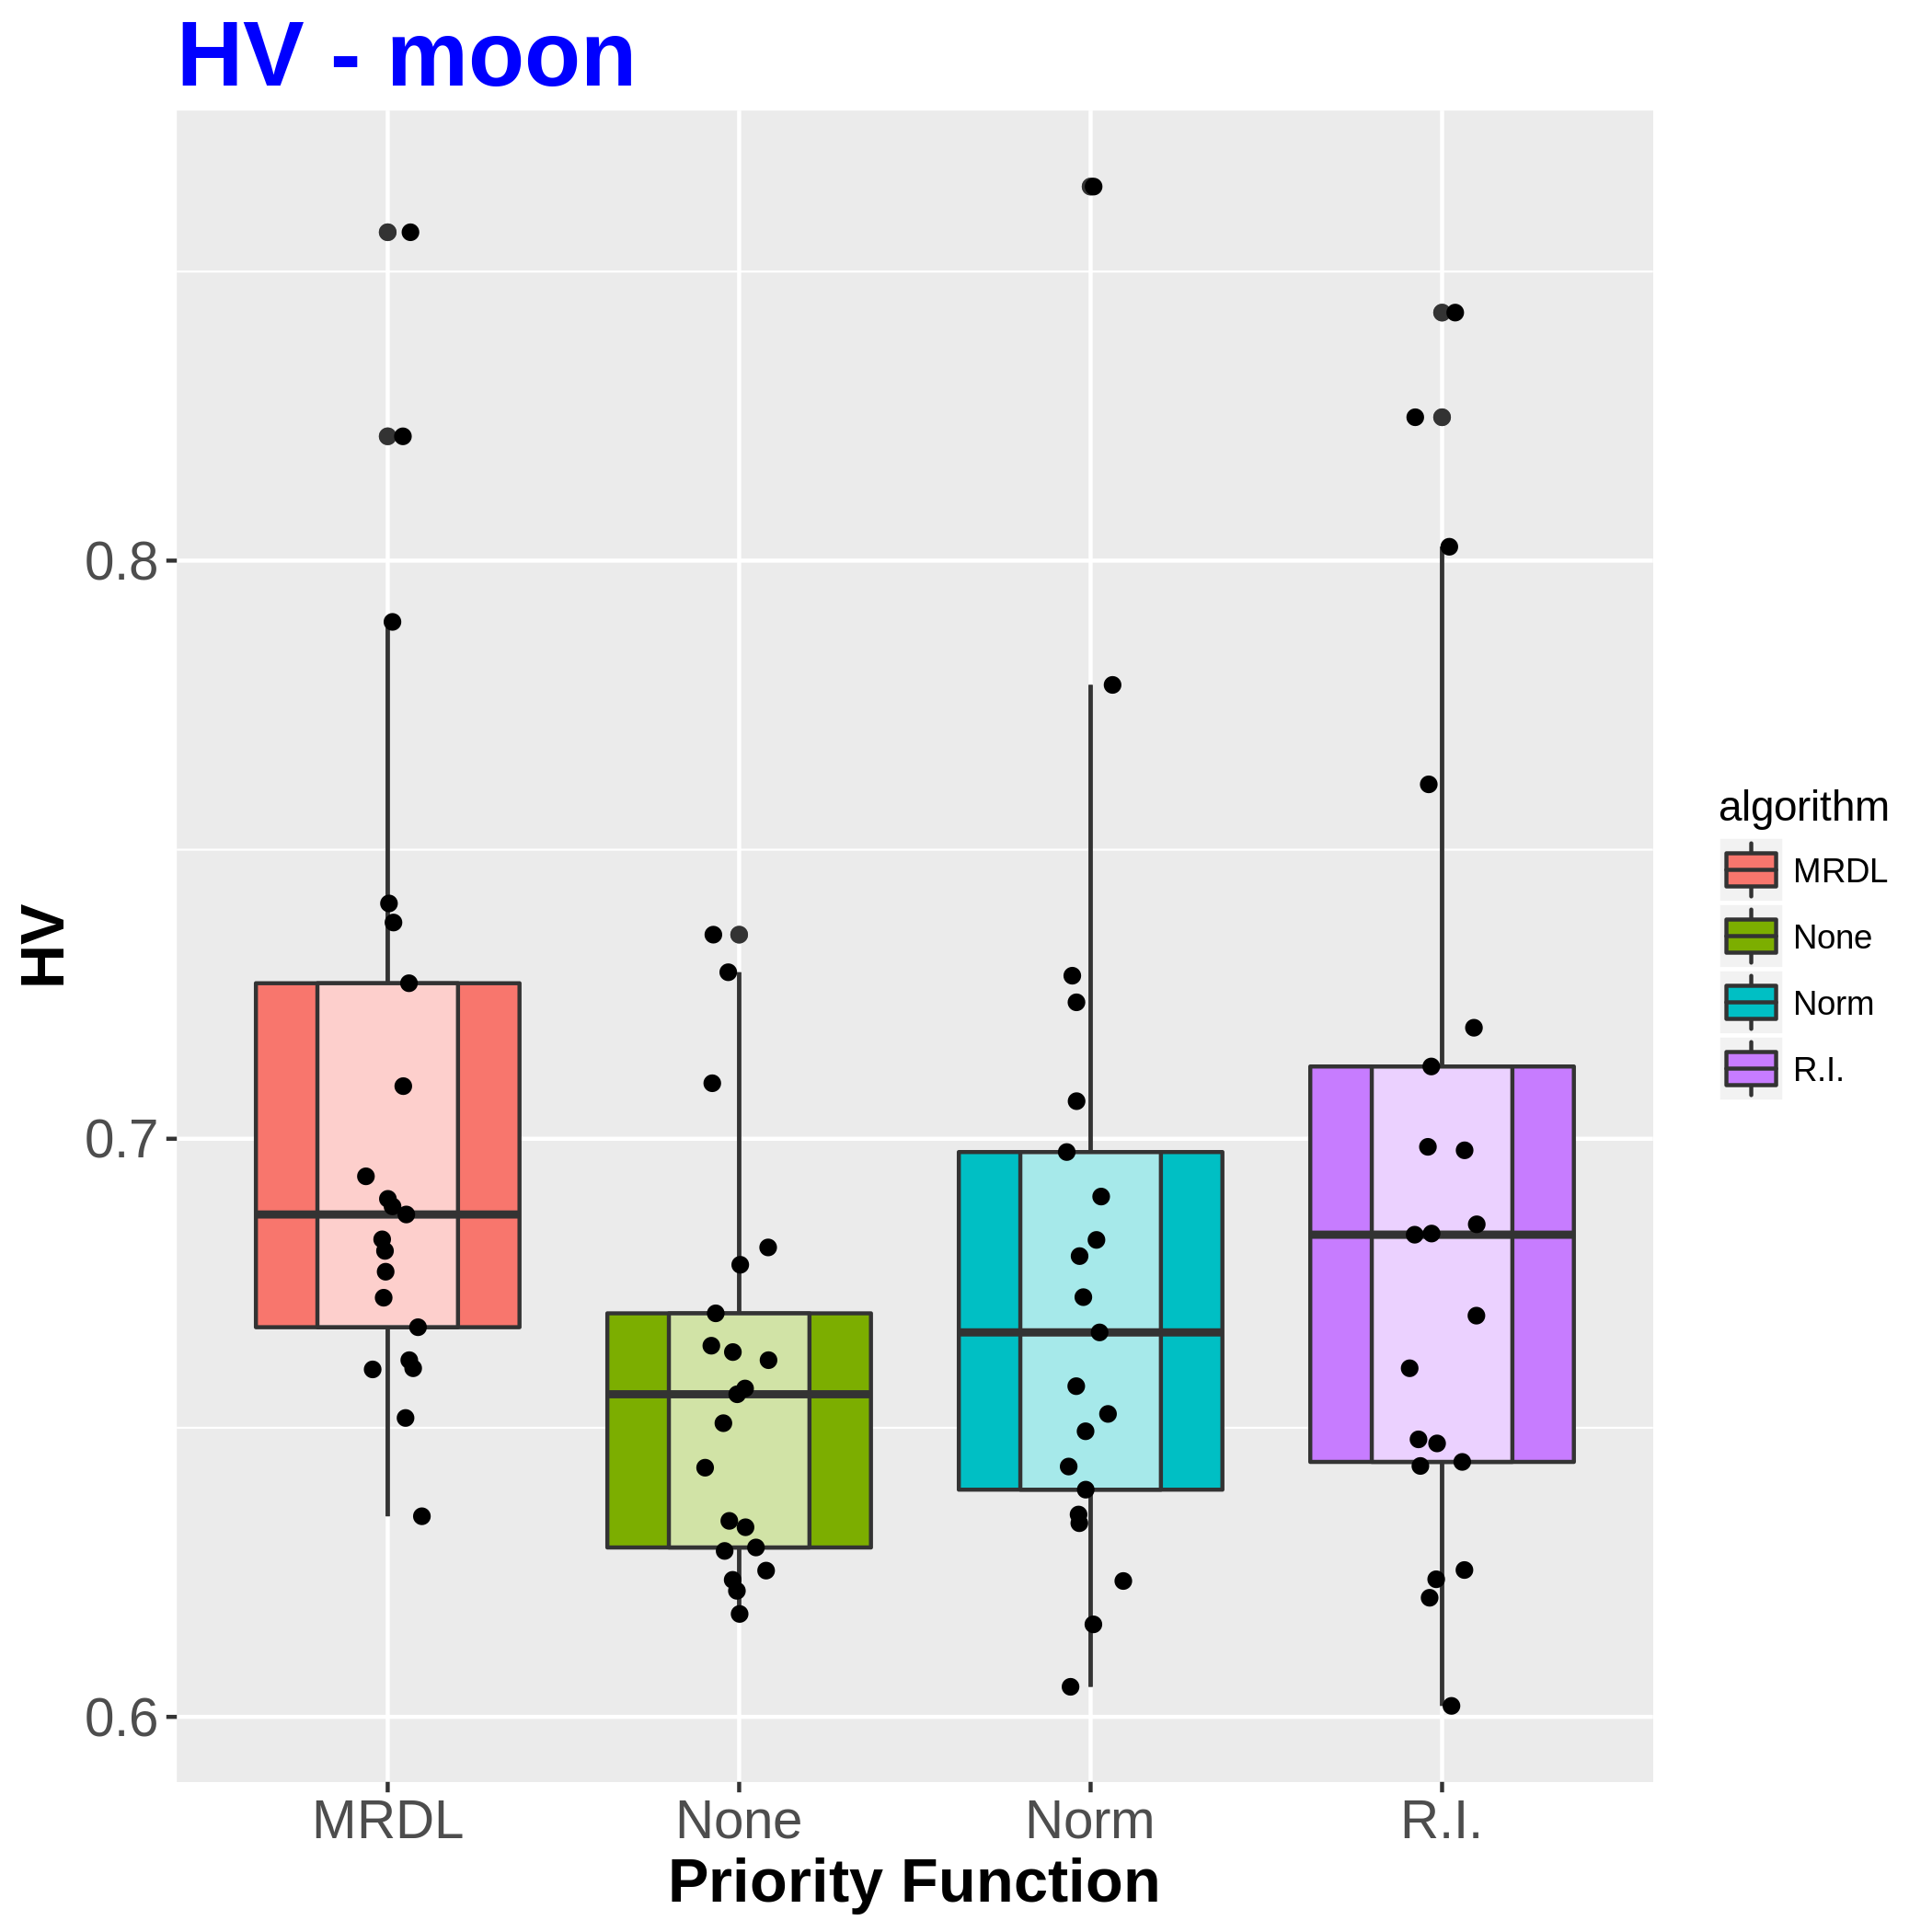
\includegraphics[width=1\textwidth, height=1\textwidth]{images/moon_HV.png}
%	\caption{HV - DTLZ4}
\end{subfigure}
	\caption{Box plot of HV values on UF9, DTLZ4 and Lunar Landing. (Higher values are better)}
		\label{HVS}
\end{figure*}

%\begin{figure*}[!t]
%%	\Large{Average performance on different tournament size - Gallagher's Gaussian 21-hi Peaks Function}
%	\begin{subfigure}[b]{0.33\textwidth}
%		\centering
%		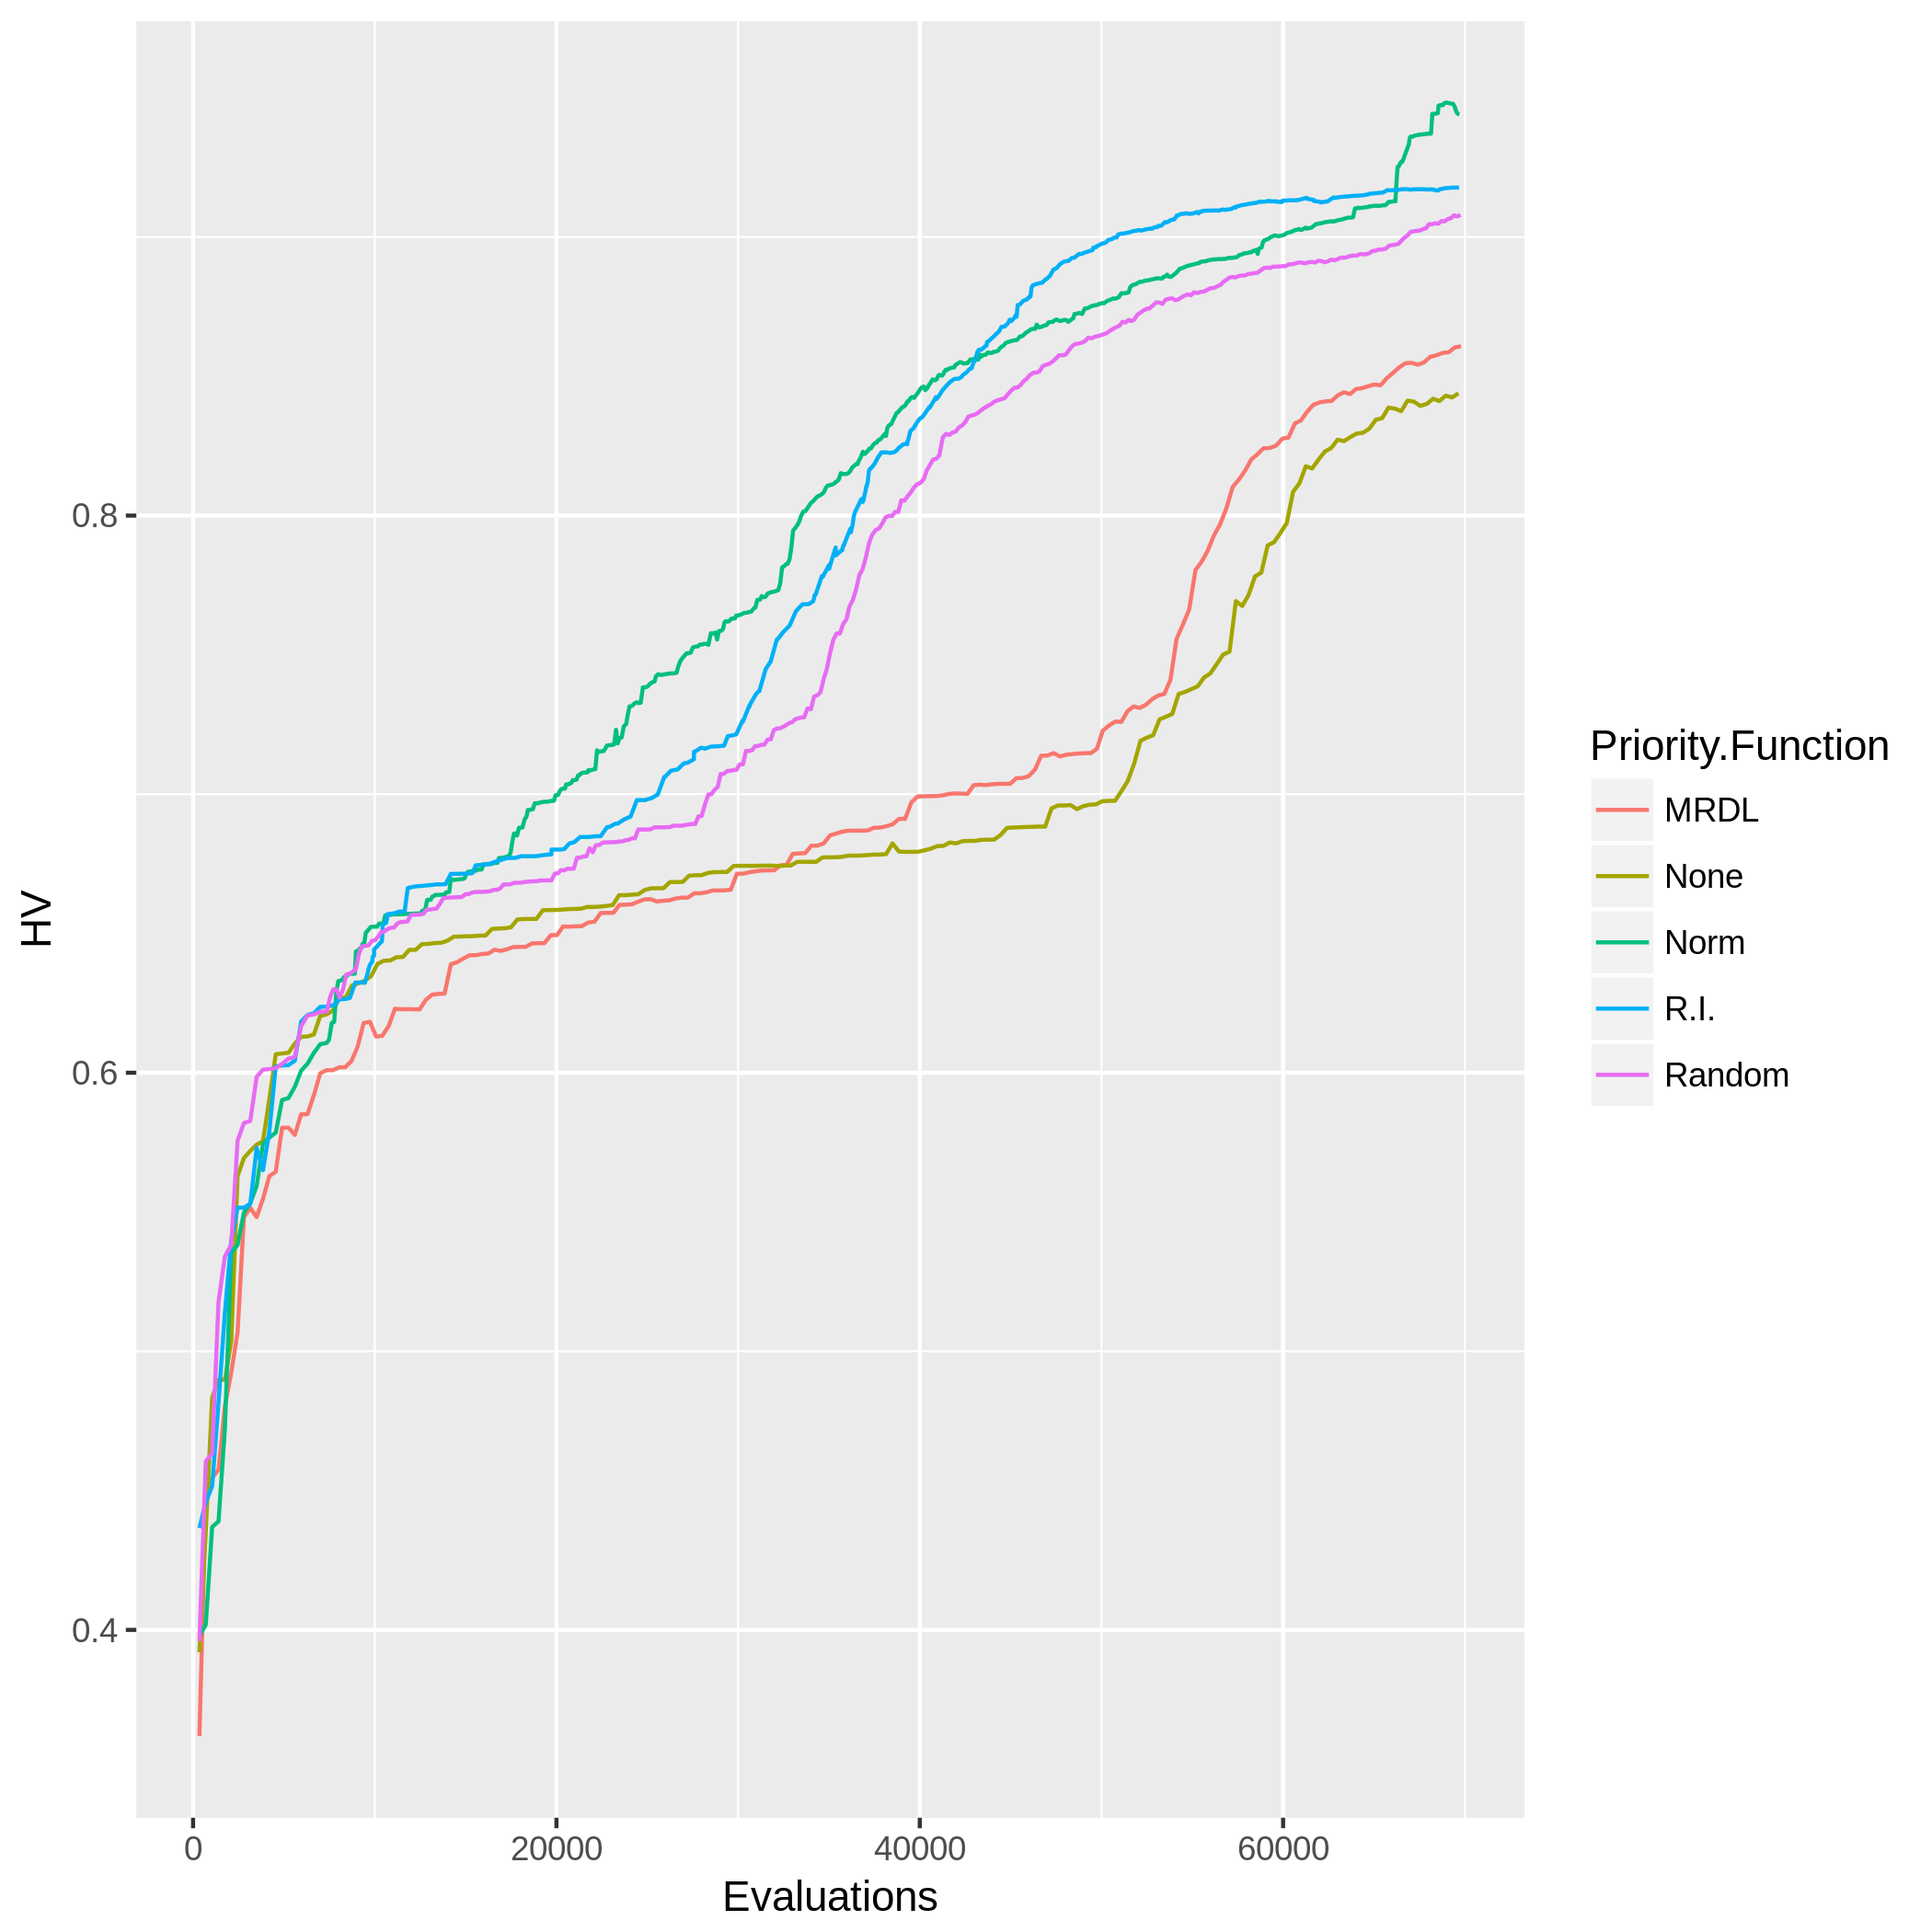
\includegraphics[width=1\textwidth, height=1\textwidth]{images/UF3hv_all}
%	\caption{Evolution - UF3}
%	\end{subfigure}
%	\begin{subfigure}[b]{0.33\textwidth}
%		\centering
%		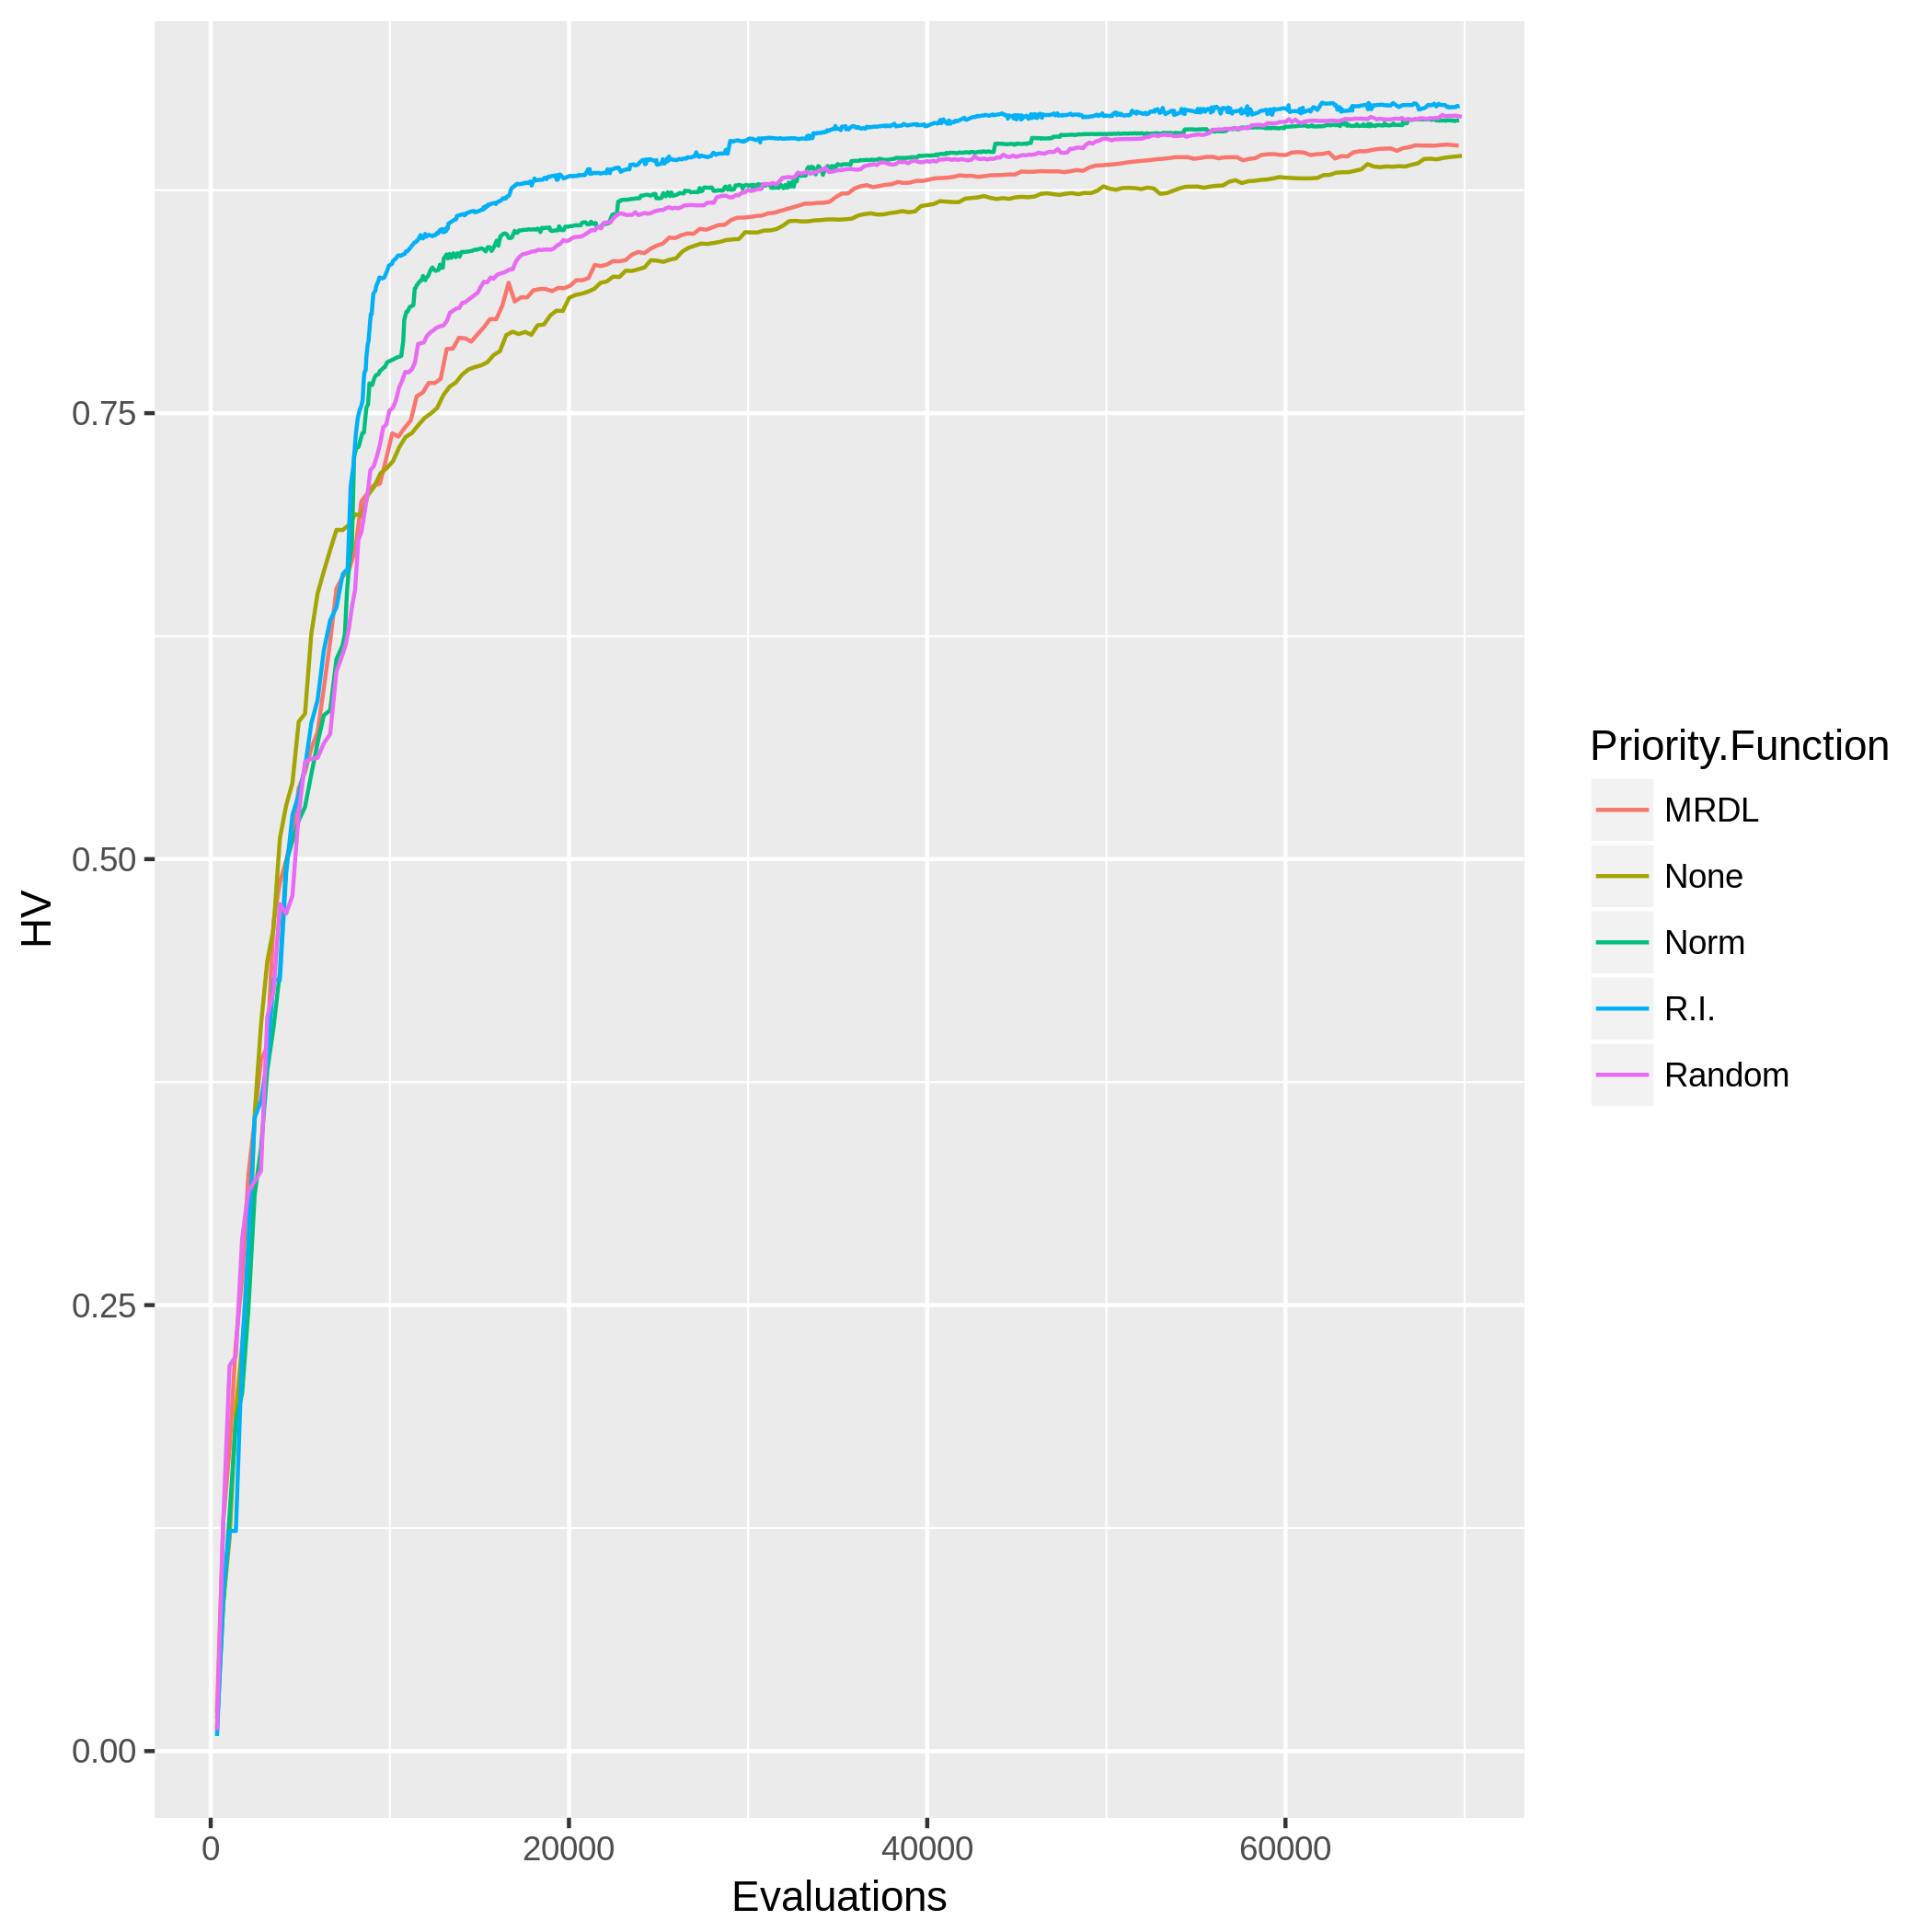
\includegraphics[width=1\textwidth, height=1\textwidth]{images/UF8hv_all}
%	\caption{Evolution - UF8}
%	\end{subfigure}
%\begin{subfigure}[b]{0.33\textwidth}
%	\centering
%	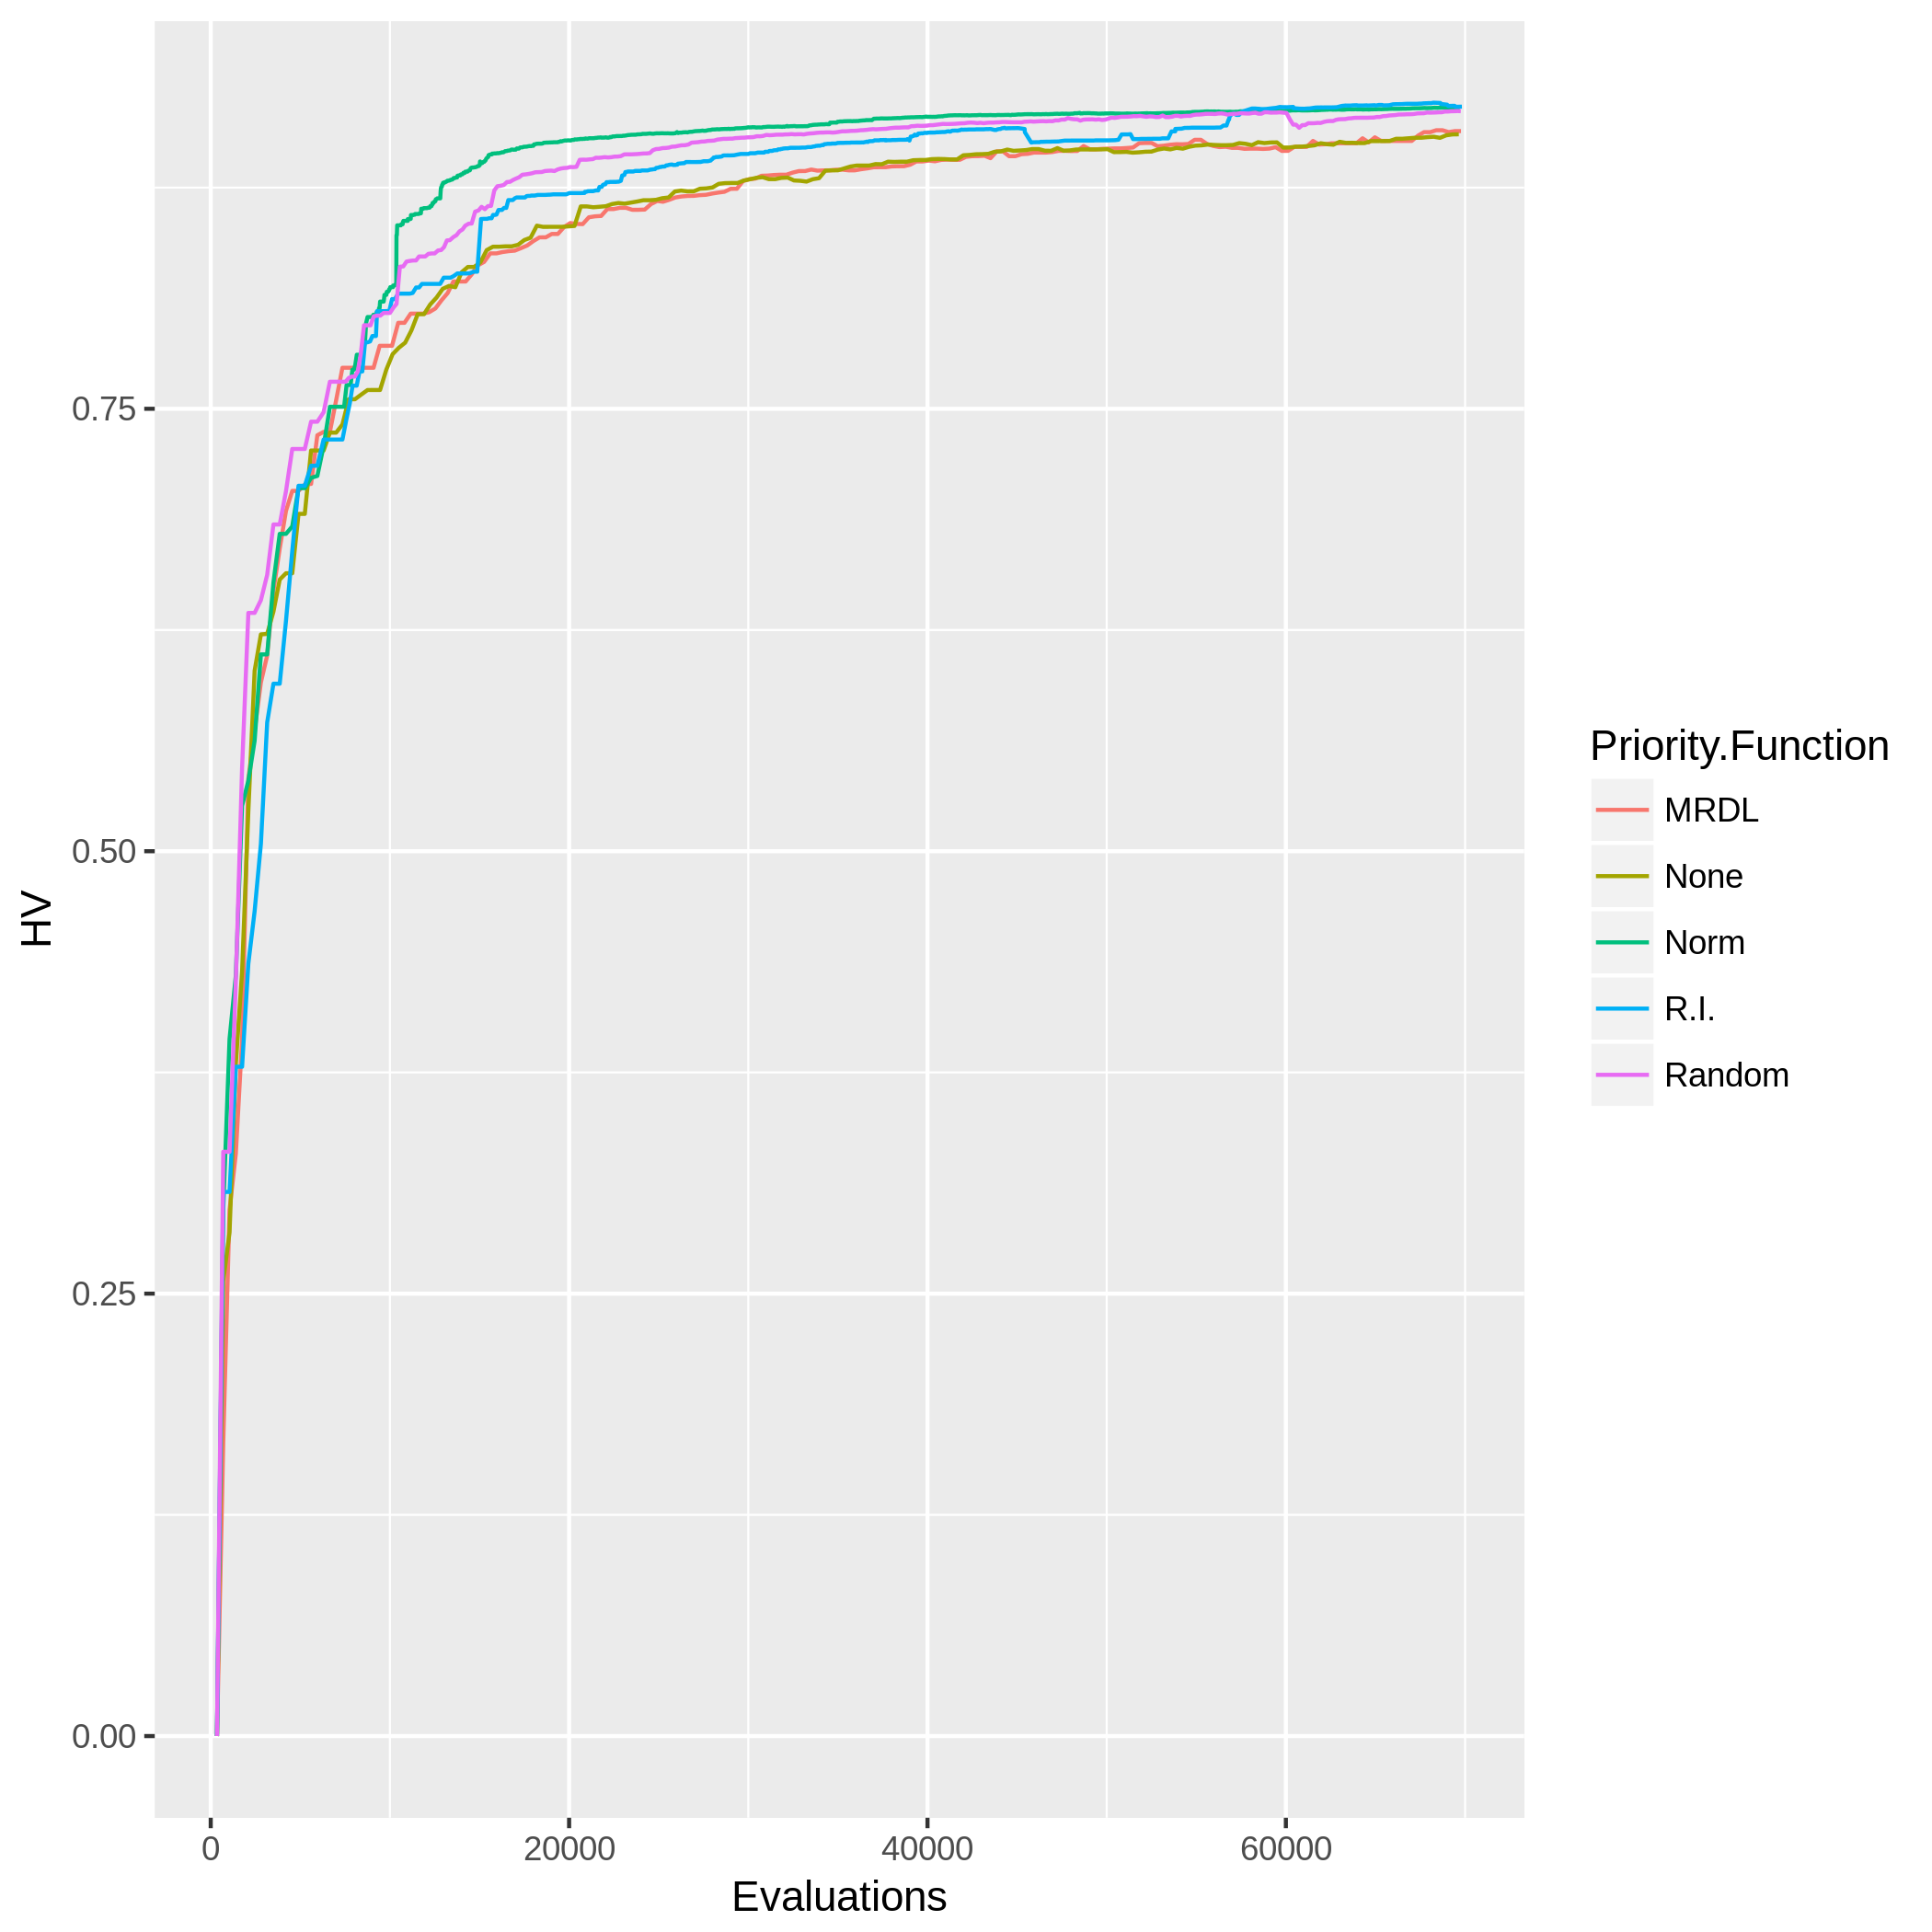
\includegraphics[width=1\textwidth, height=1\textwidth]{images/DTLZ4hv_all}
%	\caption{Evolution - DTLZ4}
%\end{subfigure}
%	\caption{Evolution of HV values on Artificial Benchmark Problems}
%\label{evolution_hv}
%\end{figure*}

\begin{figure*}[!t]

	\begin{subfigure}[b]{0.33\textwidth}
		\centering
		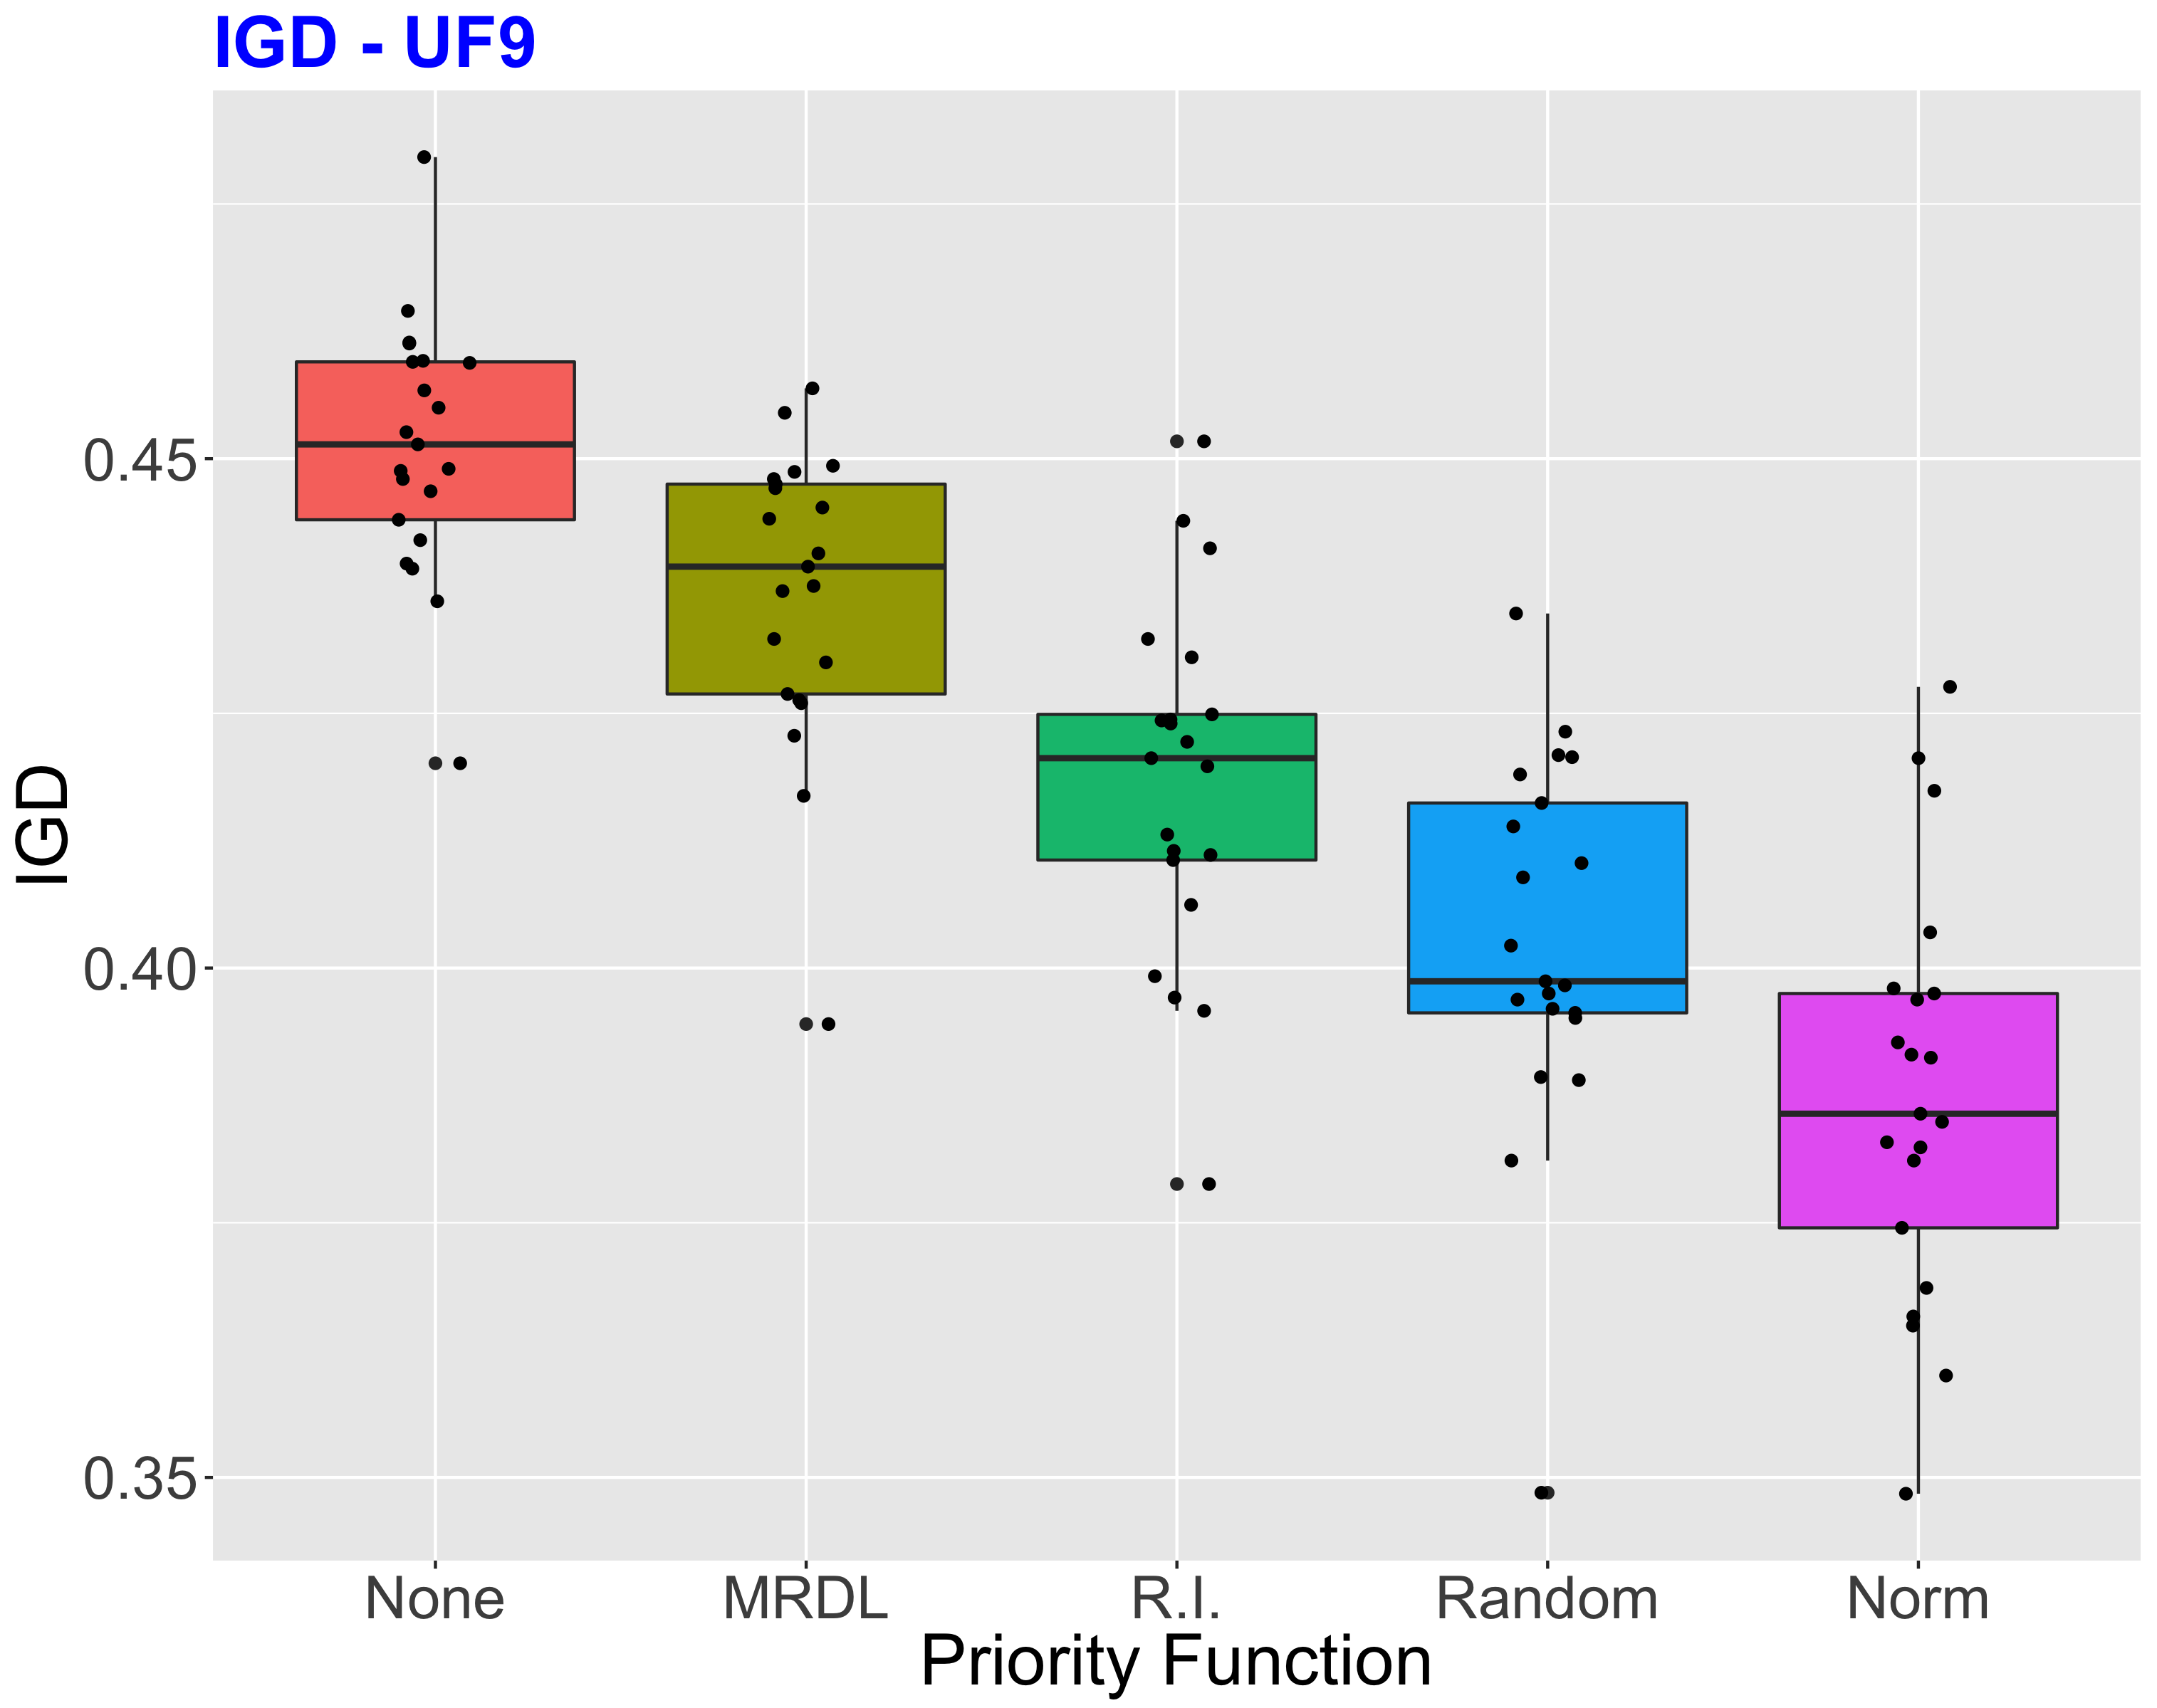
\includegraphics[width=1\textwidth, height=1\textwidth]{images/UF9_IGD.png}
%	\caption{IGD - UF3}
	\end{subfigure}
	\begin{subfigure}[b]{0.33\textwidth}
		\centering
		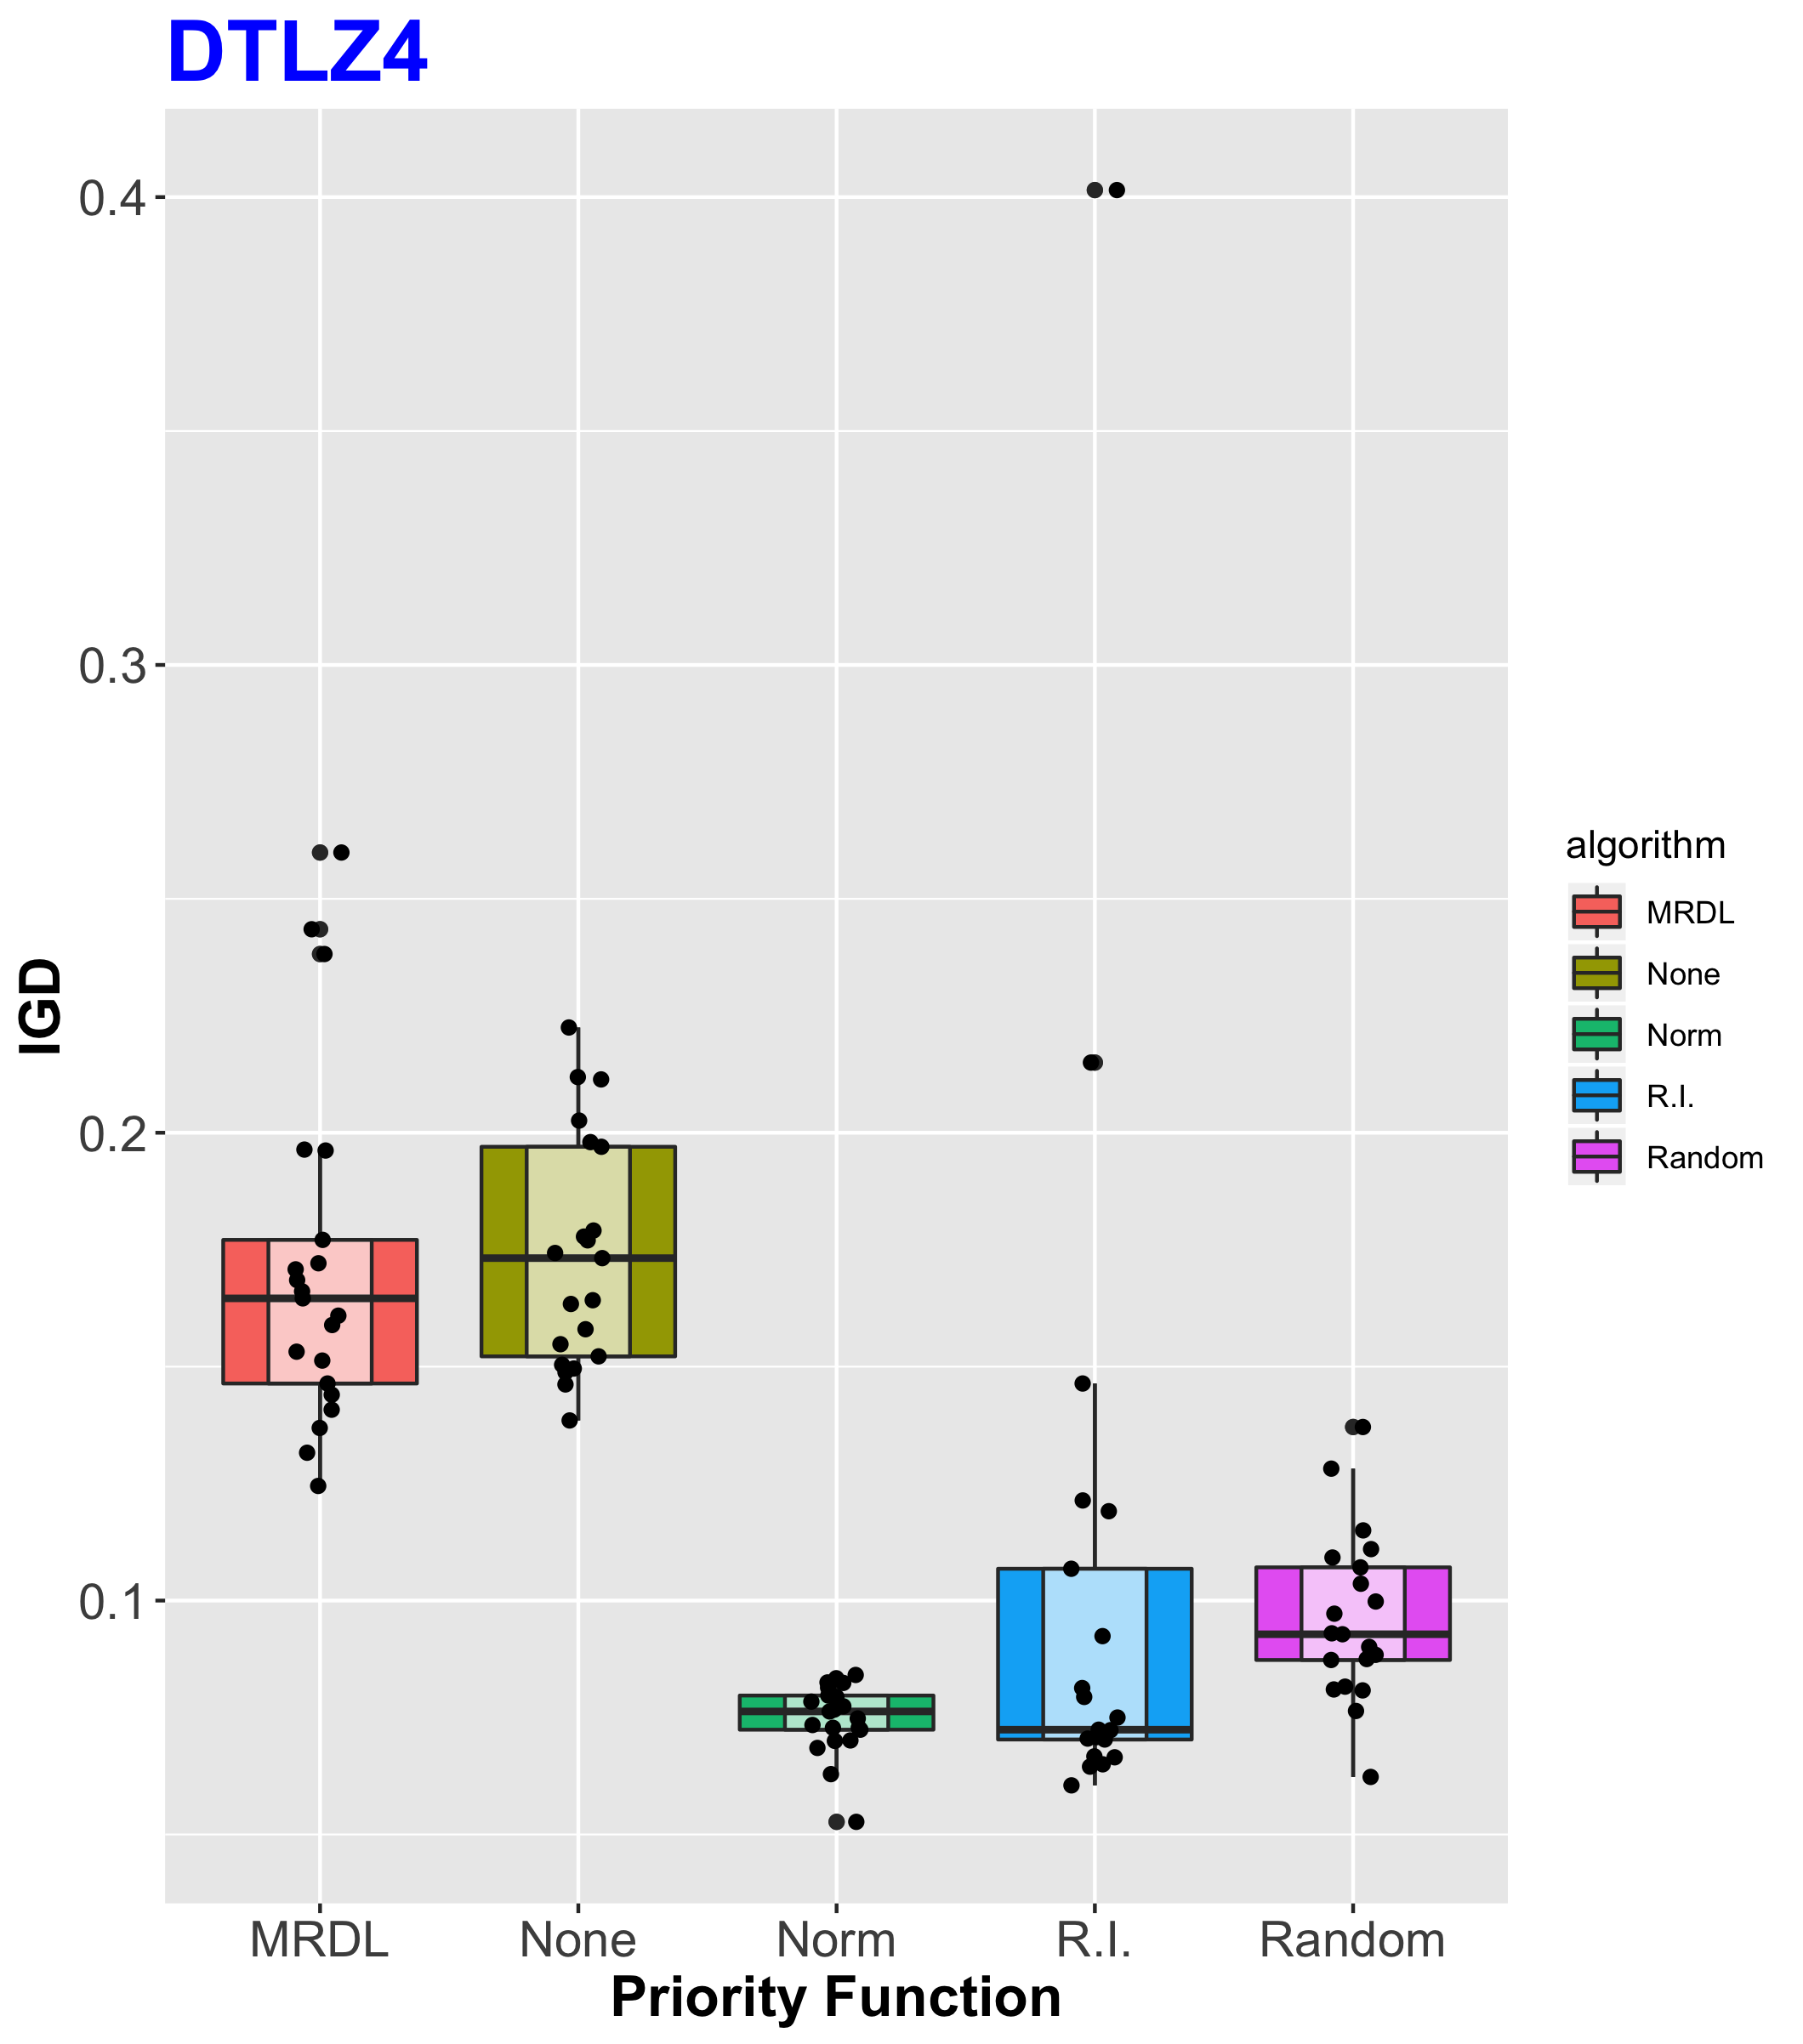
\includegraphics[width=1\textwidth, height=1\textwidth]{images/DTLZ4_IGD.png}
%	\caption{IGD - UF8}
	\end{subfigure}
%\begin{subfigure}[b]{0.33\textwidth}
%	\centering
%	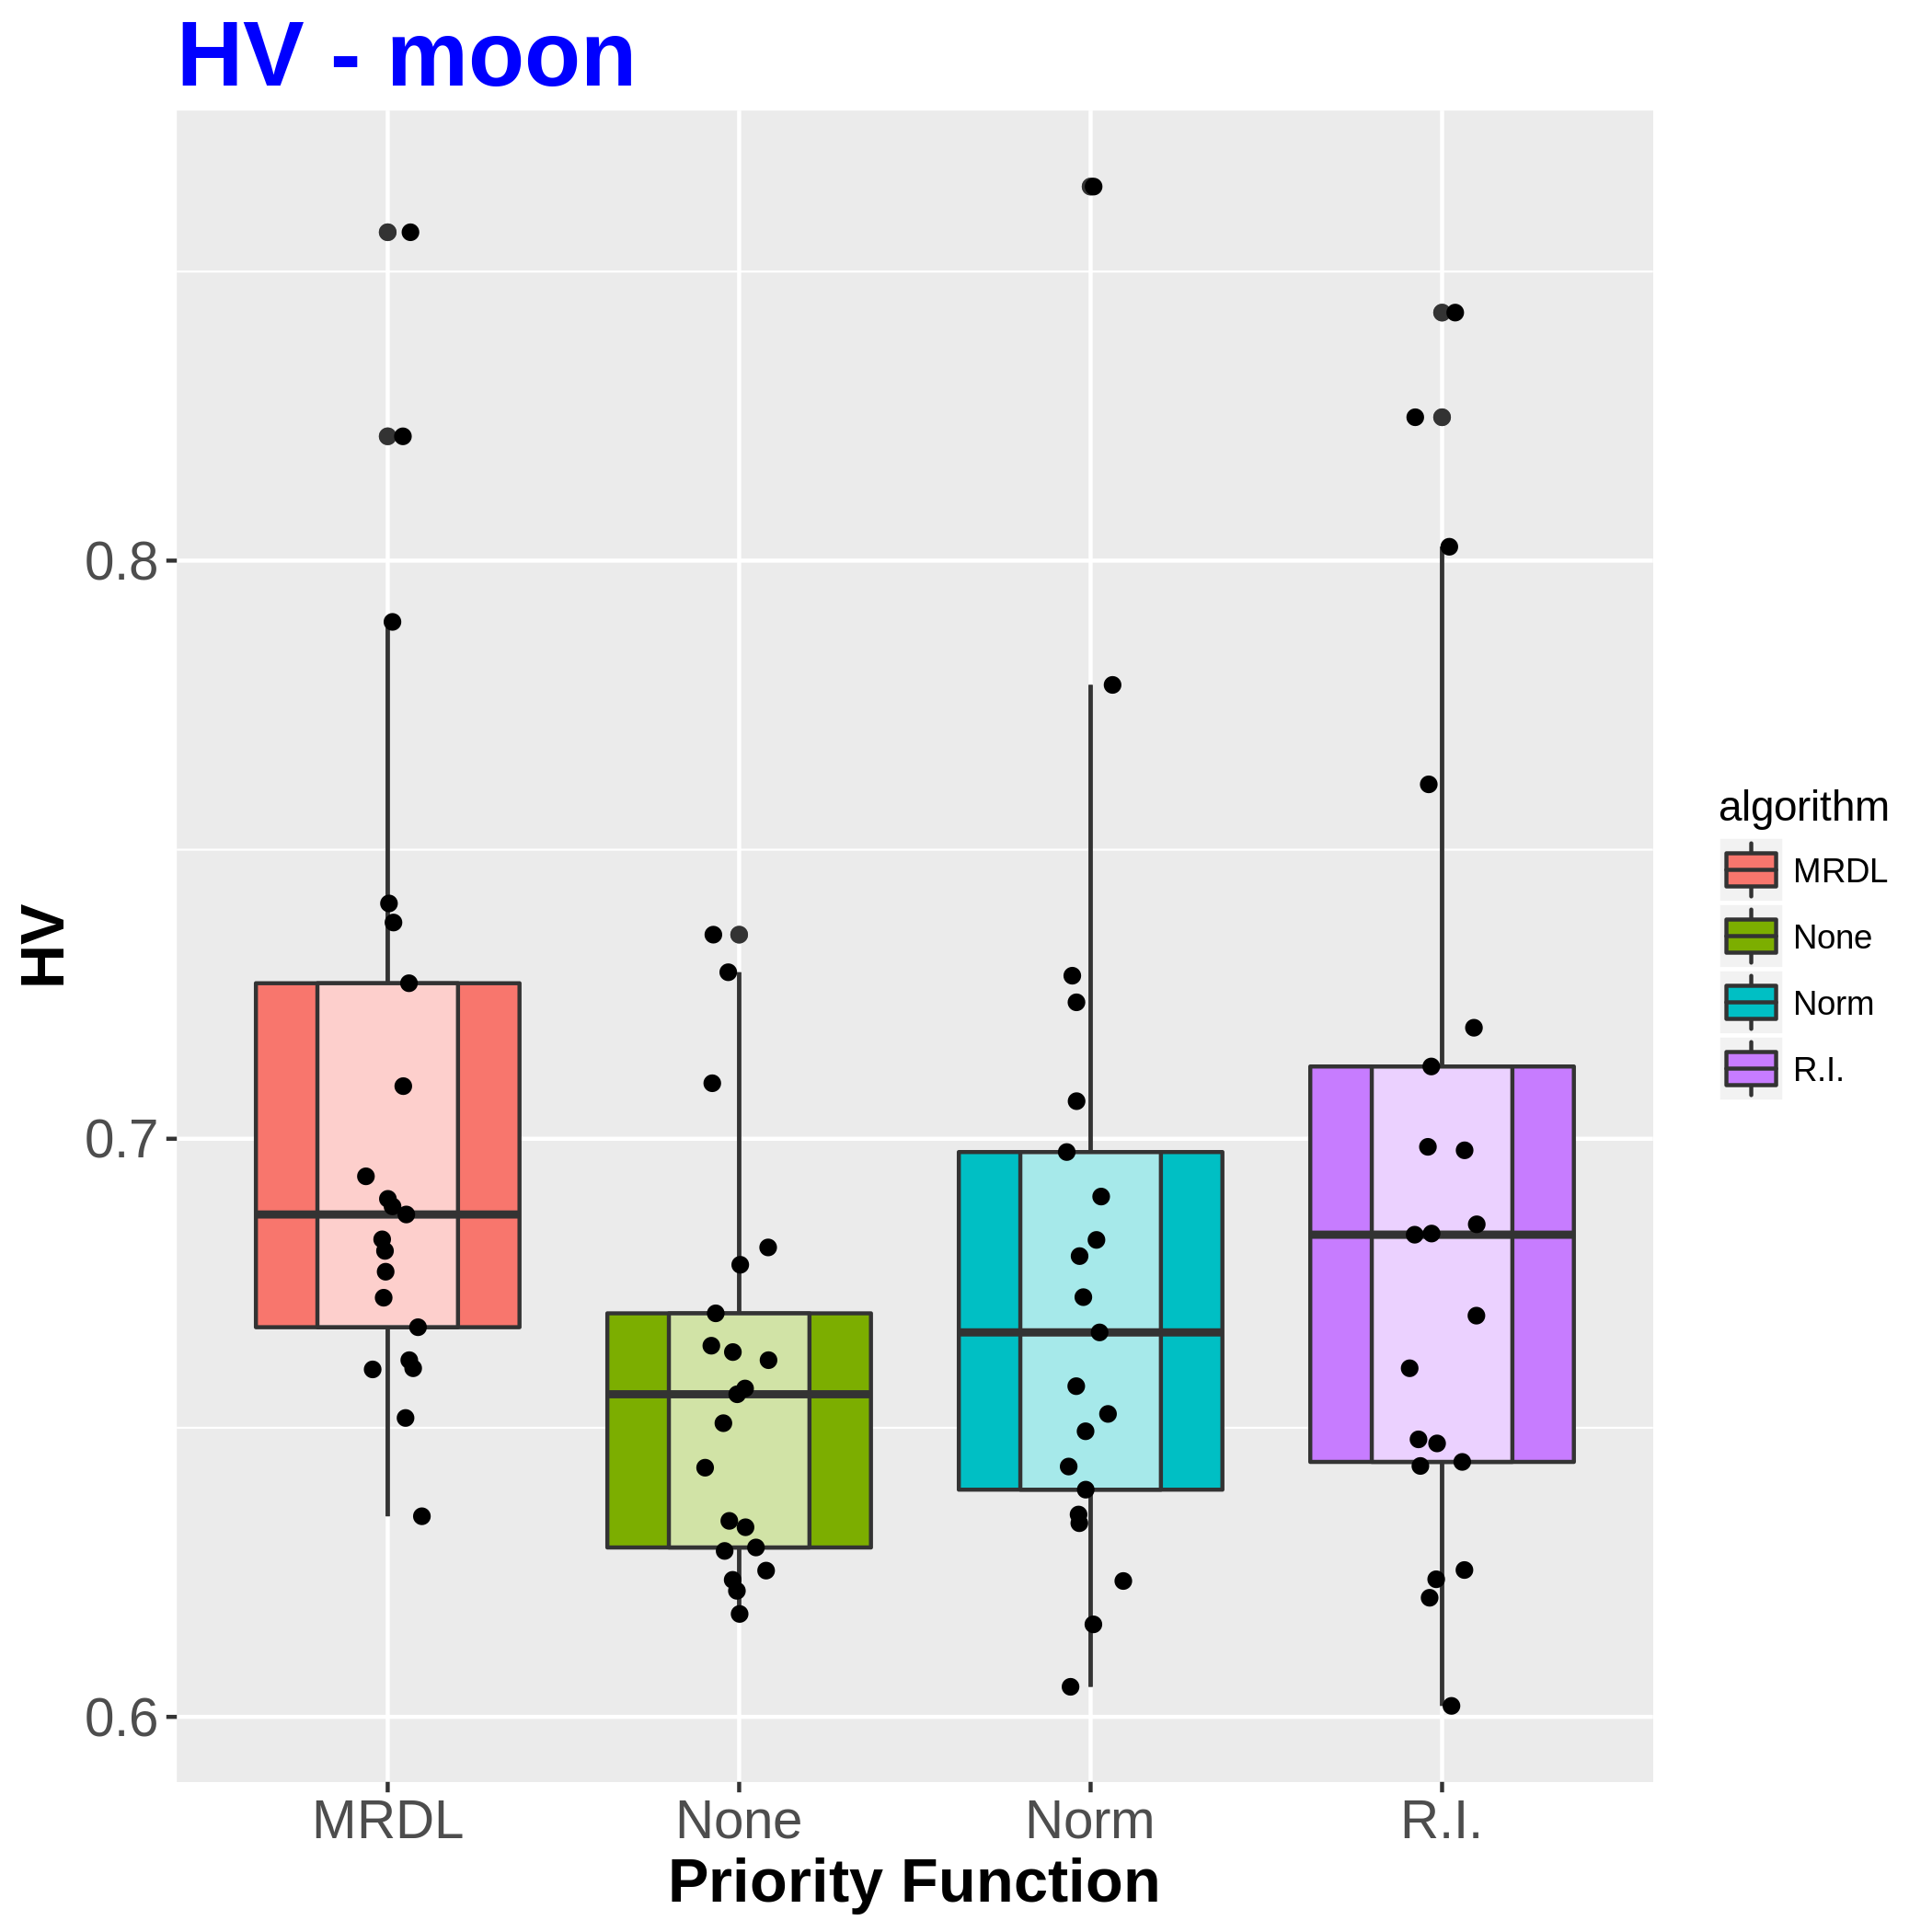
\includegraphics[width=1\textwidth, height=0.8\textwidth]{images/moon_HV}
%%	\caption{IGD - DTLZ4}
%\end{subfigure}
	\caption{Box plot of IGD values on UF9 and DTLZ4. (Lower values are better)}
		\label{IGDS}
\end{figure*}


%
%\begin{figure*}[!t]
%
%		\begin{subfigure}[b]{0.33\textwidth}
%			\centering
%		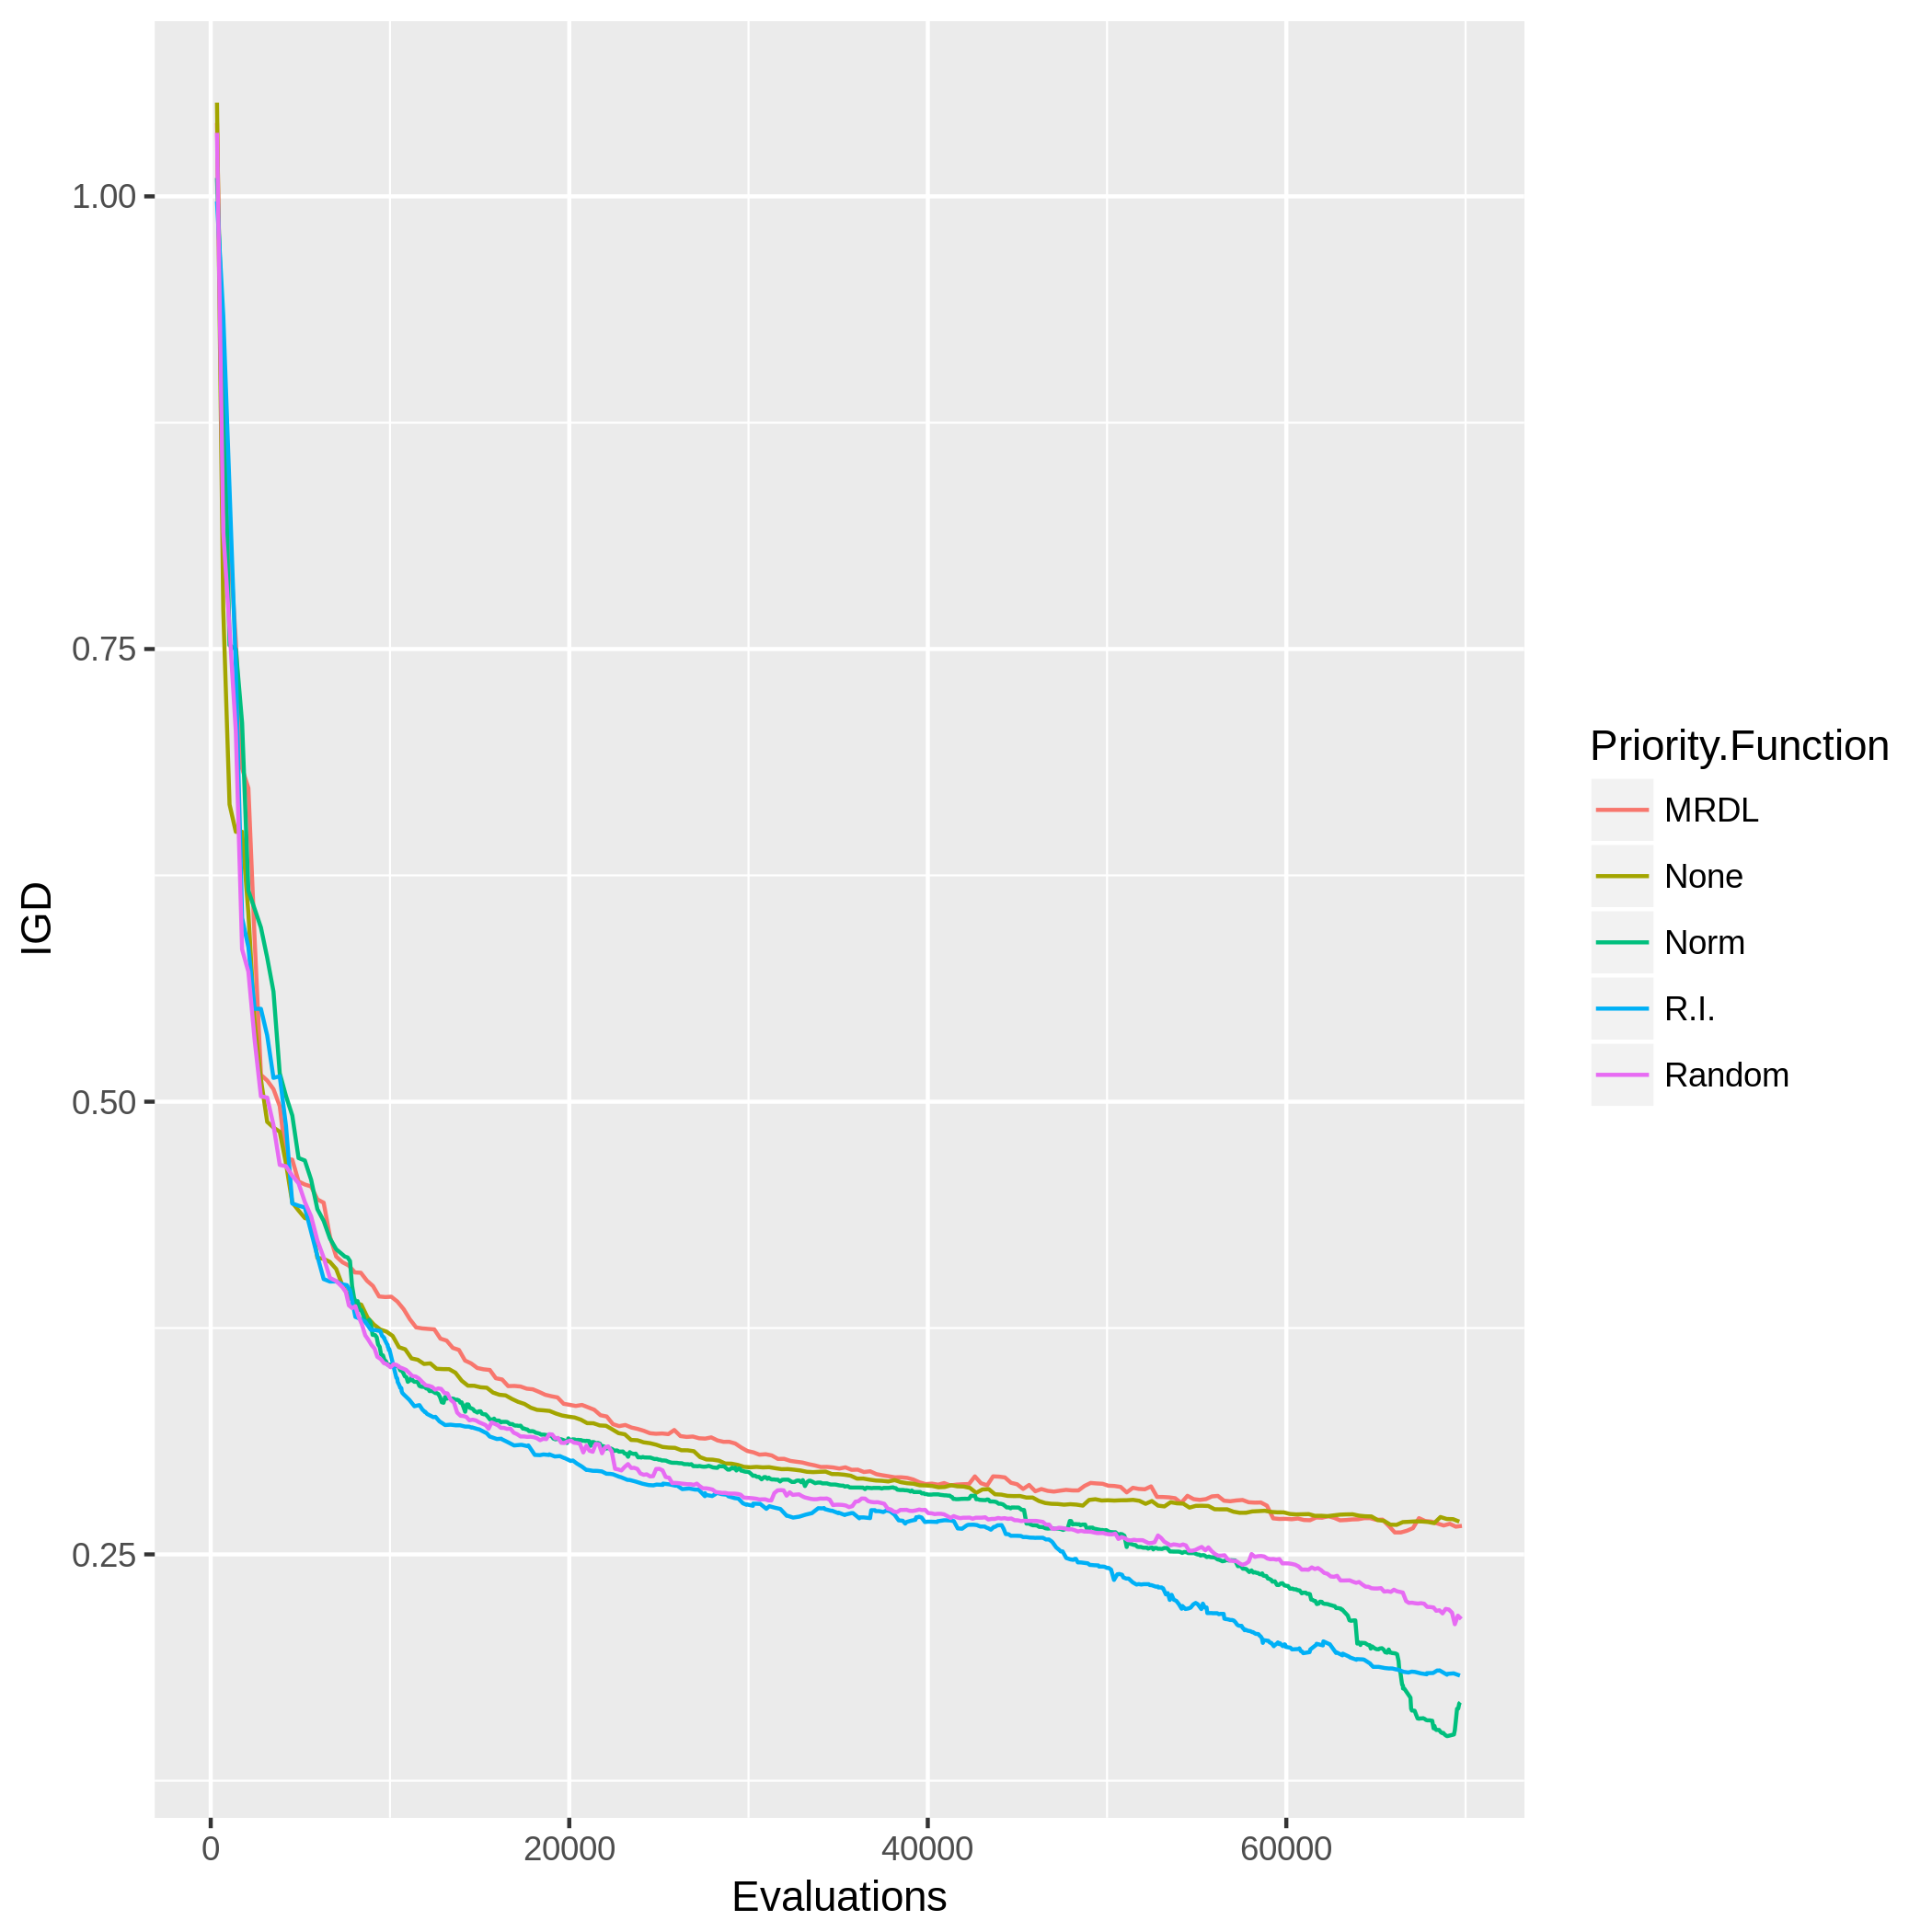
\includegraphics[width=1\textwidth, height=1\textwidth]{images/UF3igd_all}
%	\caption{Evolution - UF3}
%		\end{subfigure}
%		\begin{subfigure}[b]{0.33\textwidth}
%			\centering
%		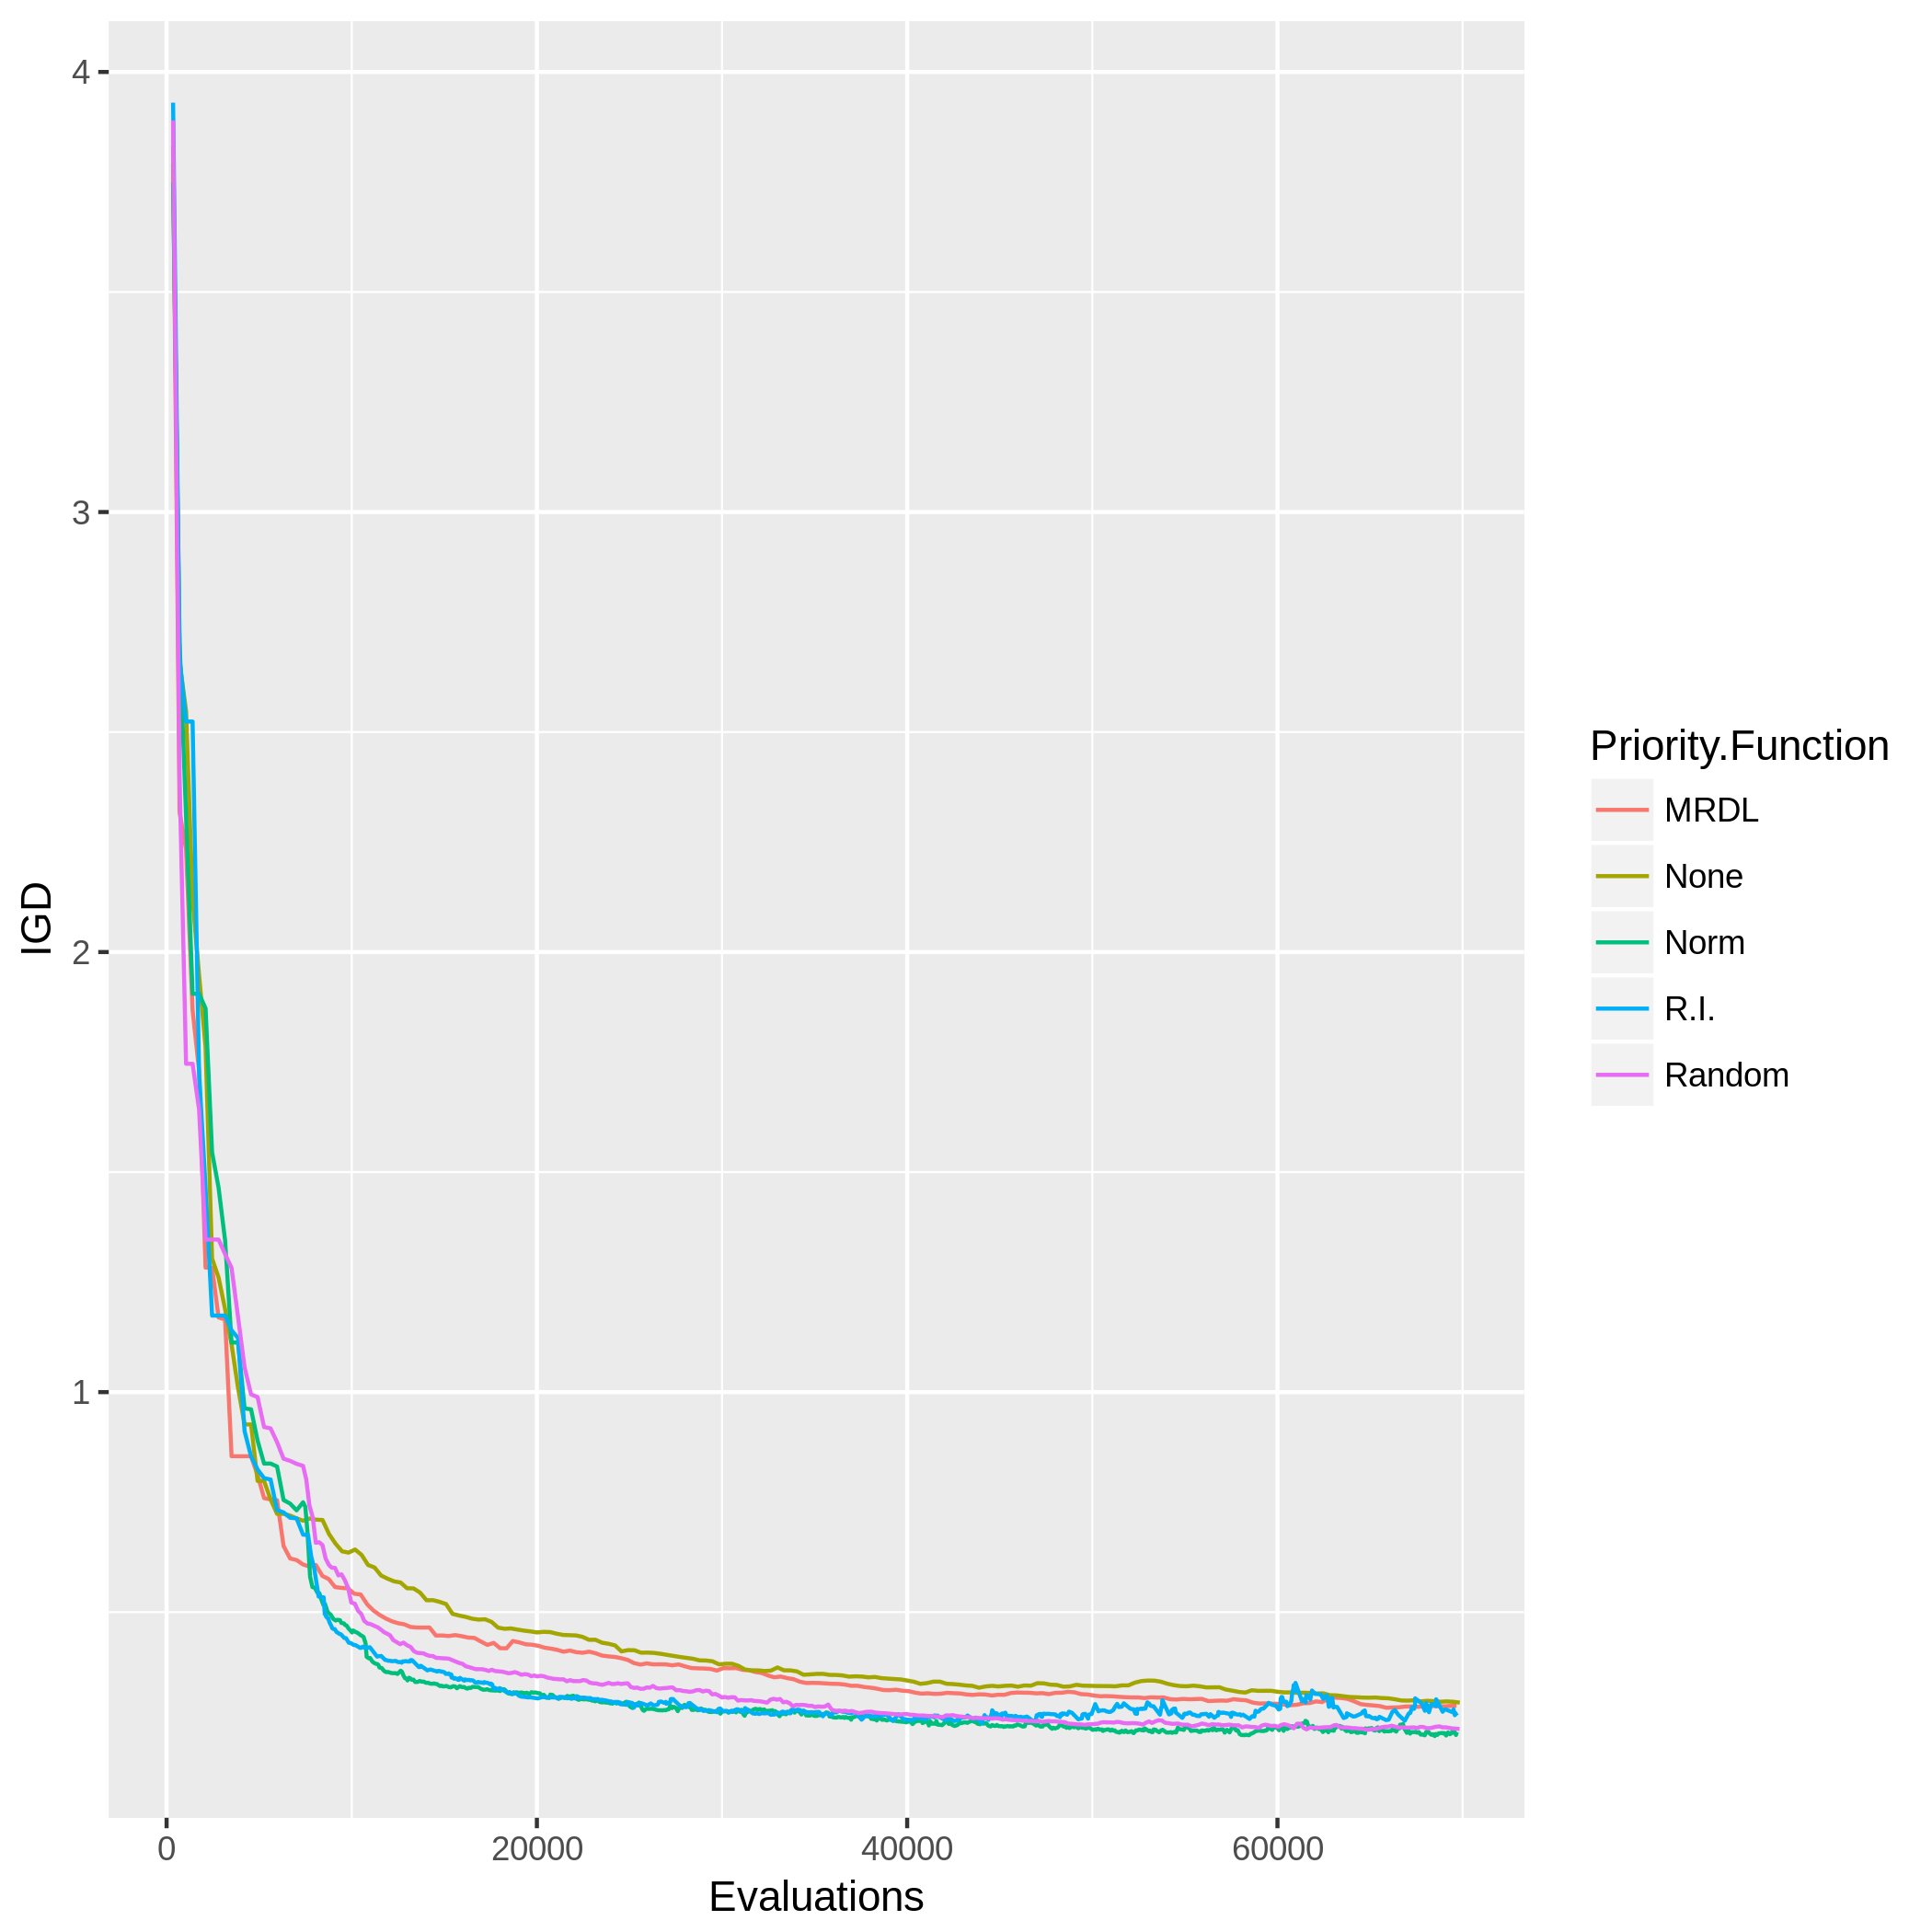
\includegraphics[width=1\textwidth, height=1\textwidth]{images/UF8igd_all}
%	\caption{Evolution - UF8}
%		\end{subfigure}
%	\begin{subfigure}[b]{0.33\textwidth}
%		\centering
%		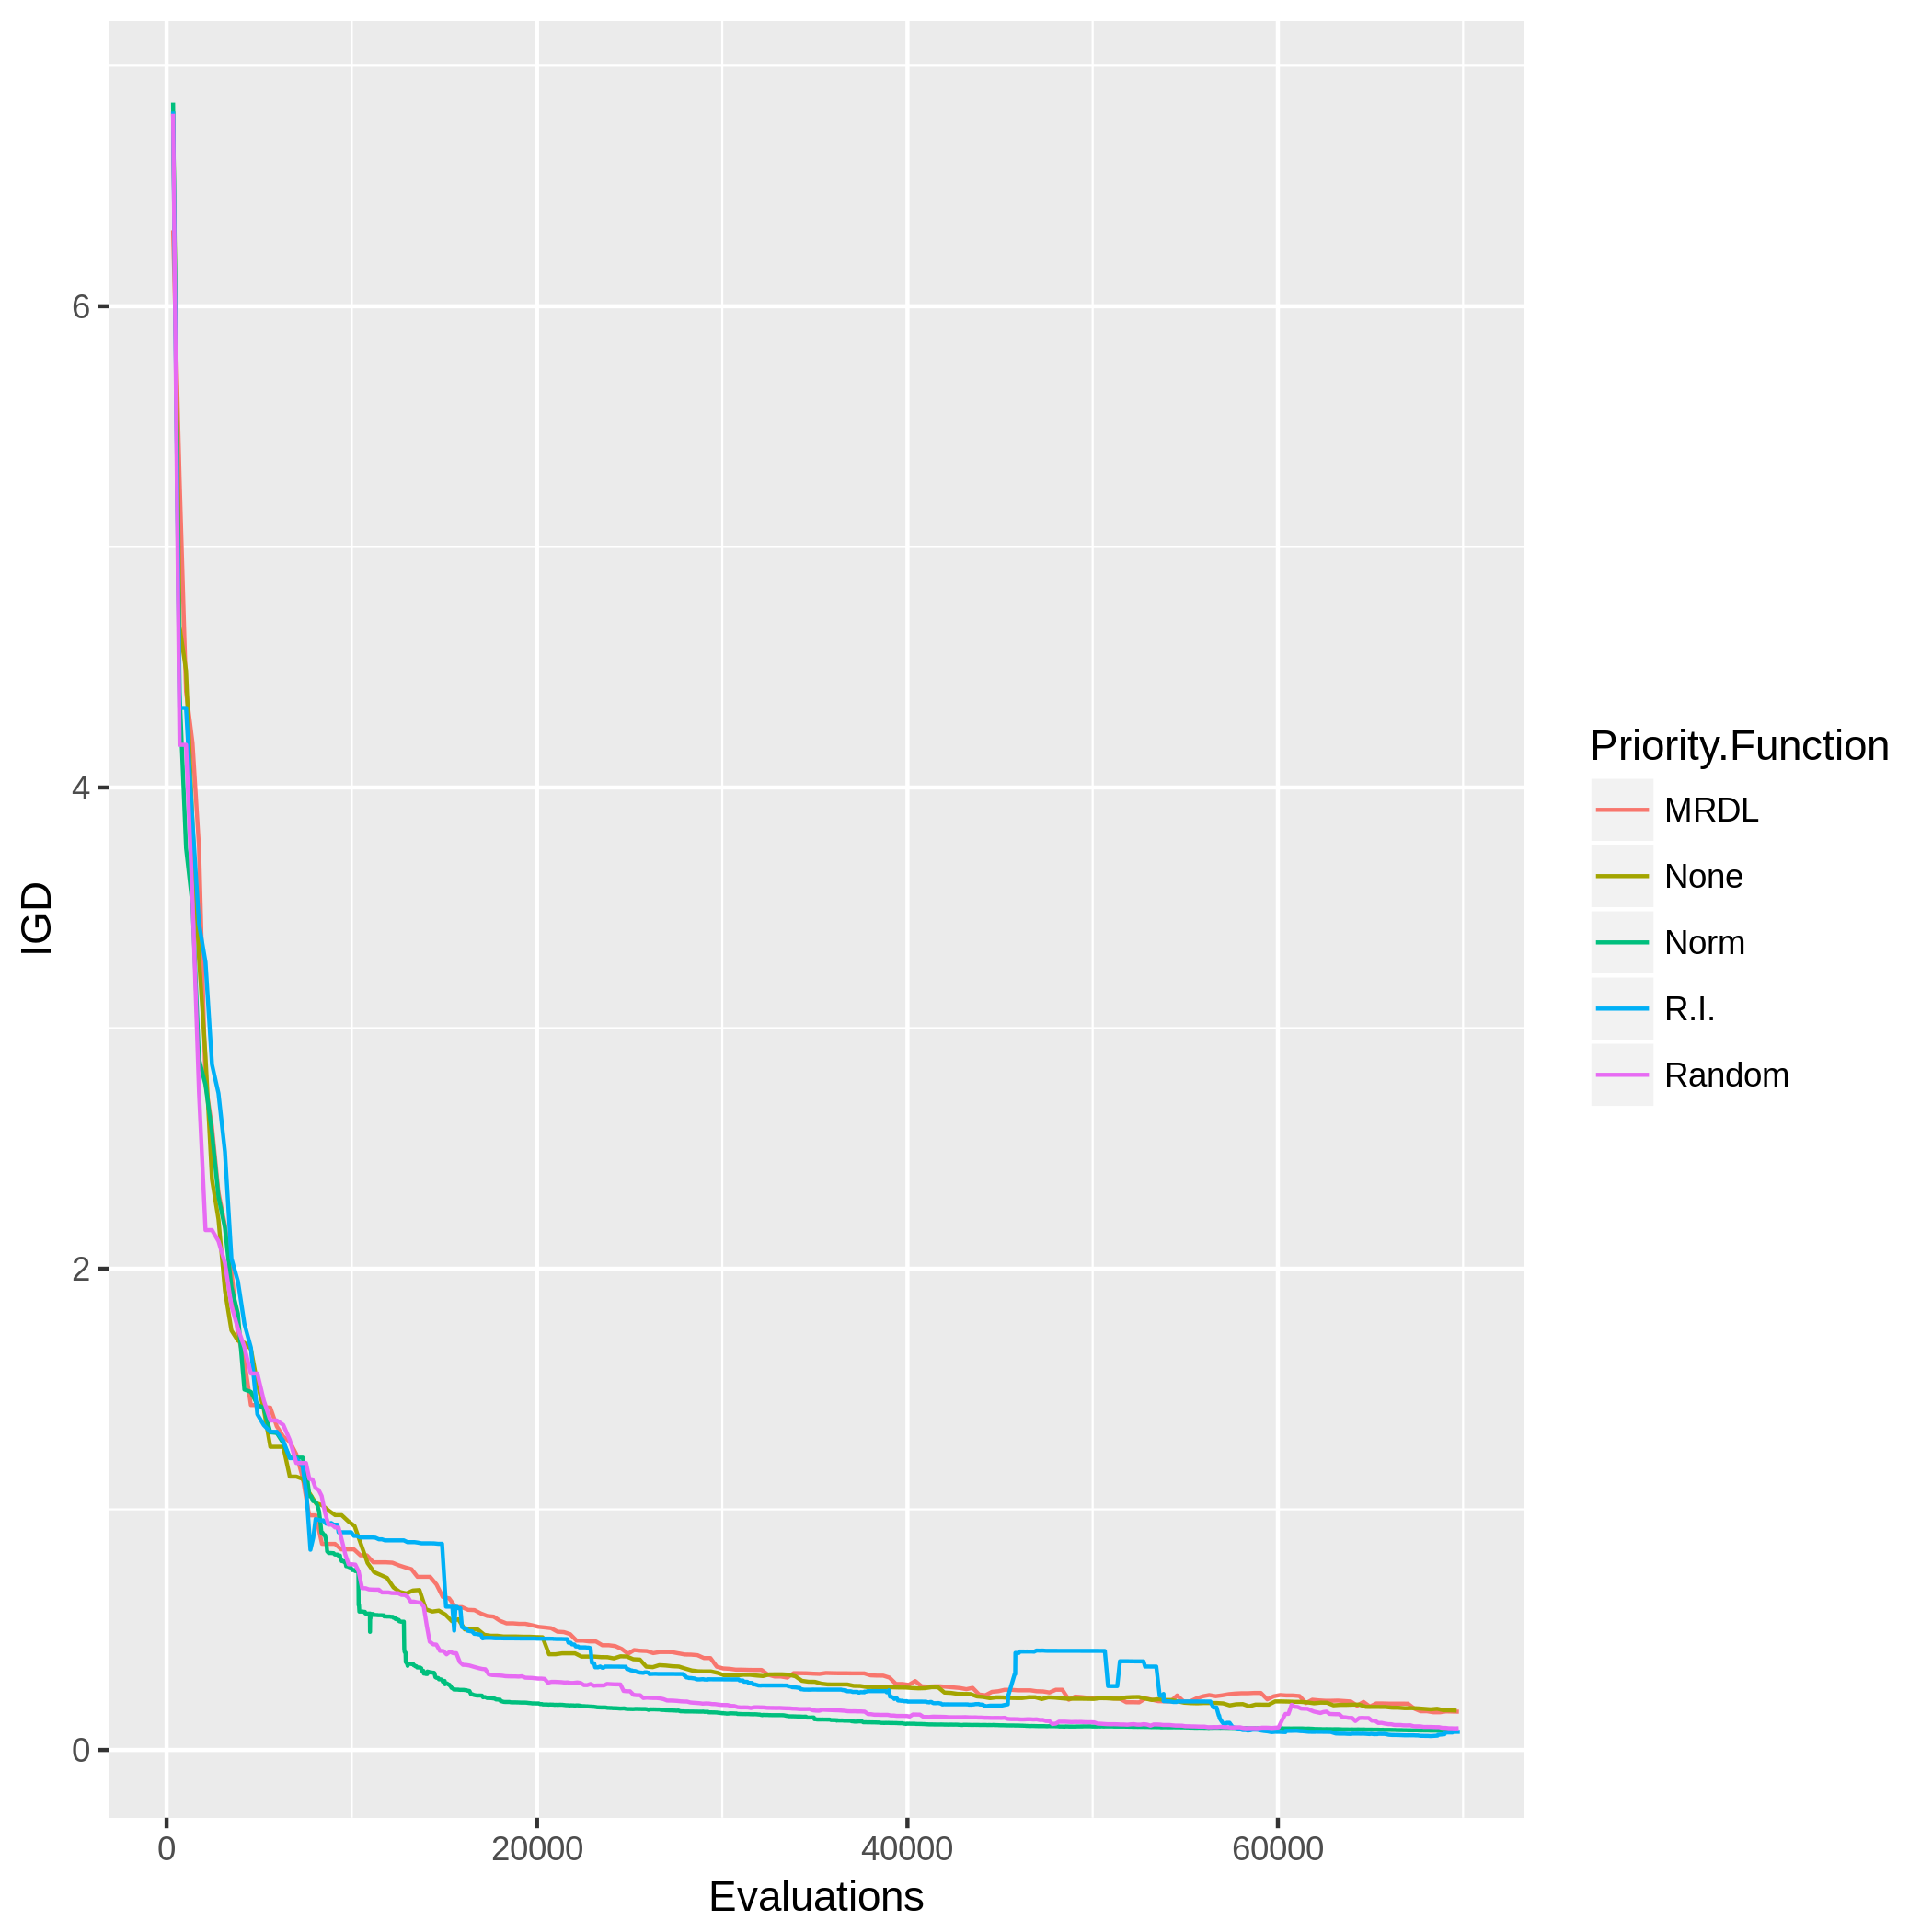
\includegraphics[width=1\textwidth, height=1\textwidth]{images/DTLZ4igd_all}
%	\caption{Evolution - DTLZ4}
%	\end{subfigure}
%	\caption{Evolution of HV values on Artificial Benchmark Problems}
%			\label{evolution_igd}
%	\end{figure*}

\begin{figure}[!t]

	%	\Large{Average performance on different tournament size - Gallagher's Gaussian 21-hi Peaks Function}
	%	\begin{subfigure}[b]{0.33\textwidth}
	\centering
	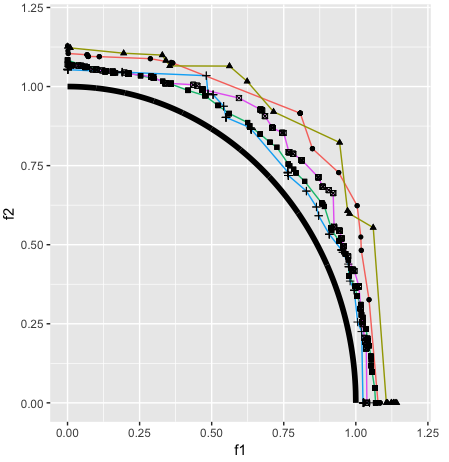
\includegraphics[width=0.43\textwidth, height=0.33\textwidth]{images/Pareto-front-dtlz4.png}
	%		\caption{RA- UF8}
	%	\end{subfigure}
	\caption{Pareto Front approximations of all priority functions and None on DTLZ4.}
	\label{PFs}

\end{figure}

\begin{figure*}[!t]

	%	\Large{Average performance on different tournament size - Gallagher's Gaussian 21-hi Peaks Function}
	\begin{subfigure}[b]{0.33\textwidth}
		\centering
		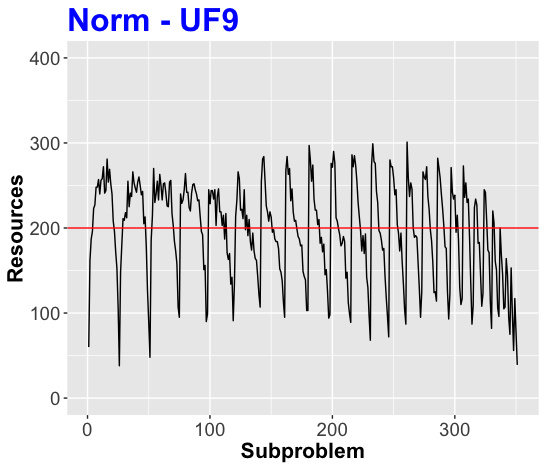
\includegraphics[width=1\textwidth, height=0.8\textwidth]{images/Ra-norm-uf9.png}
%		\caption{RA- UF8}
	\end{subfigure}
	\begin{subfigure}[b]{0.33\textwidth}
		\centering
		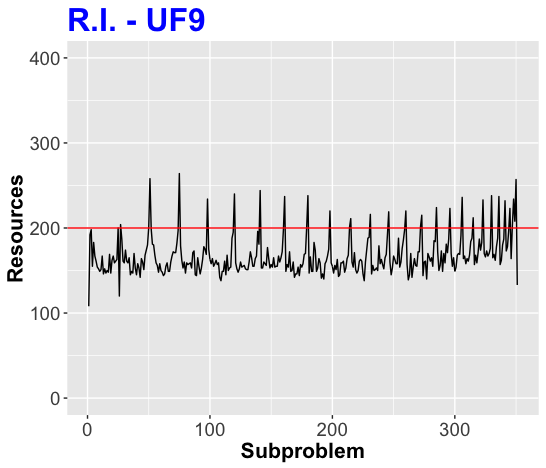
\includegraphics[width=1\textwidth, height=0.8\textwidth]{images/Ra-gra-uf9.png}
%		\caption{RA- UF8}
	\end{subfigure}
	\begin{subfigure}[b]{0.33\textwidth}
		\centering
		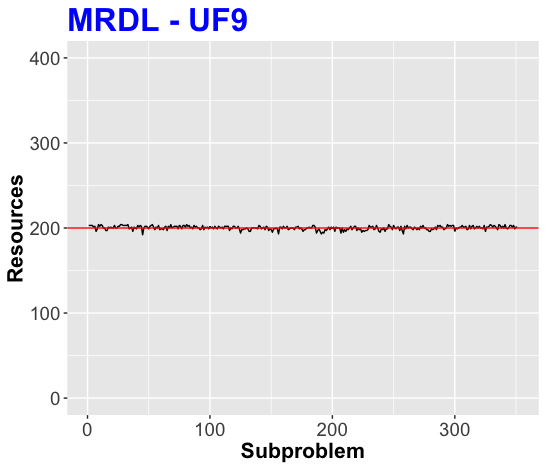
\includegraphics[width=1\textwidth, height=0.8\textwidth]{images/Ra-mrdl-uf9.png}
%		\caption{RA- UF8}
	\end{subfigure}
	\begin{subfigure}[b]{0.33\textwidth}
		\centering
		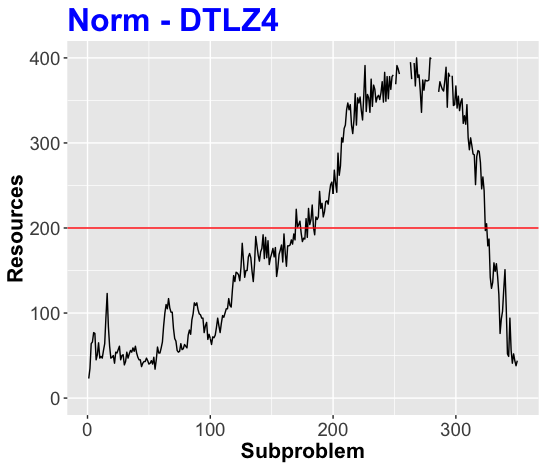
\includegraphics[width=1\textwidth, height=0.8\textwidth]{images/Ra-norm-dtlz4.png}
%		\caption{RA- UF8}
	\end{subfigure}
	\begin{subfigure}[b]{0.33\textwidth}
		\centering
		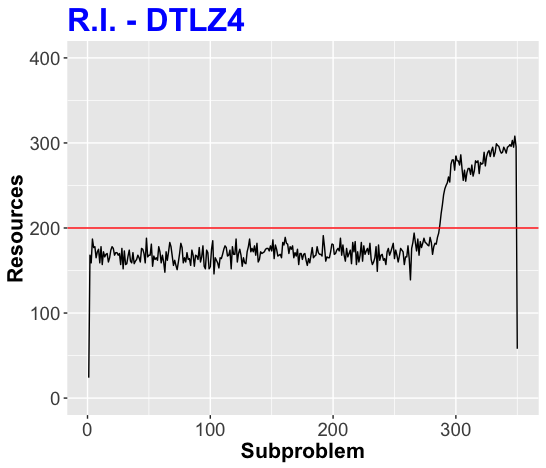
\includegraphics[width=1\textwidth, height=0.8\textwidth]{images/Ra-gra-dtlz4.png}
%		\caption{RA- UF8}
	\end{subfigure}
	\begin{subfigure}[b]{0.33\textwidth}
		\centering
		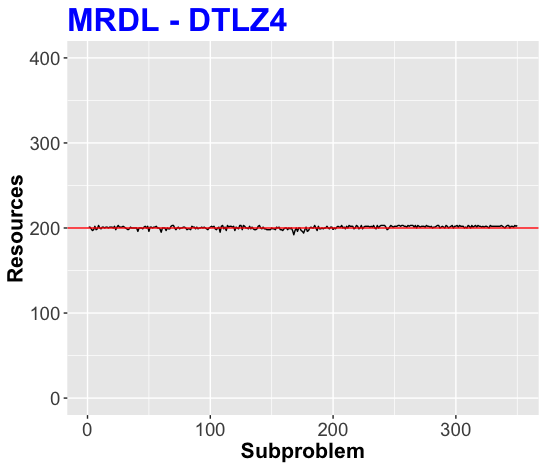
\includegraphics[width=1\textwidth, height=0.8\textwidth]{images/Ra-mrdl-dtlz4.png}
%		\caption{RA- UF8}
	\end{subfigure}
	\caption{Resource Allocation by subproblem - The red line indicates the default amount of resource for each problem, i.e., with no priority function.}
	\label{RAs}

\end{figure*}



%
%\begin{figure*}[!t]
%
%	%	\Large{Average performance on different tournament size - Gallagher's Gaussian 21-hi Peaks Function}
%	\begin{subfigure}[b]{0.33\textwidth}
%		\centering
%		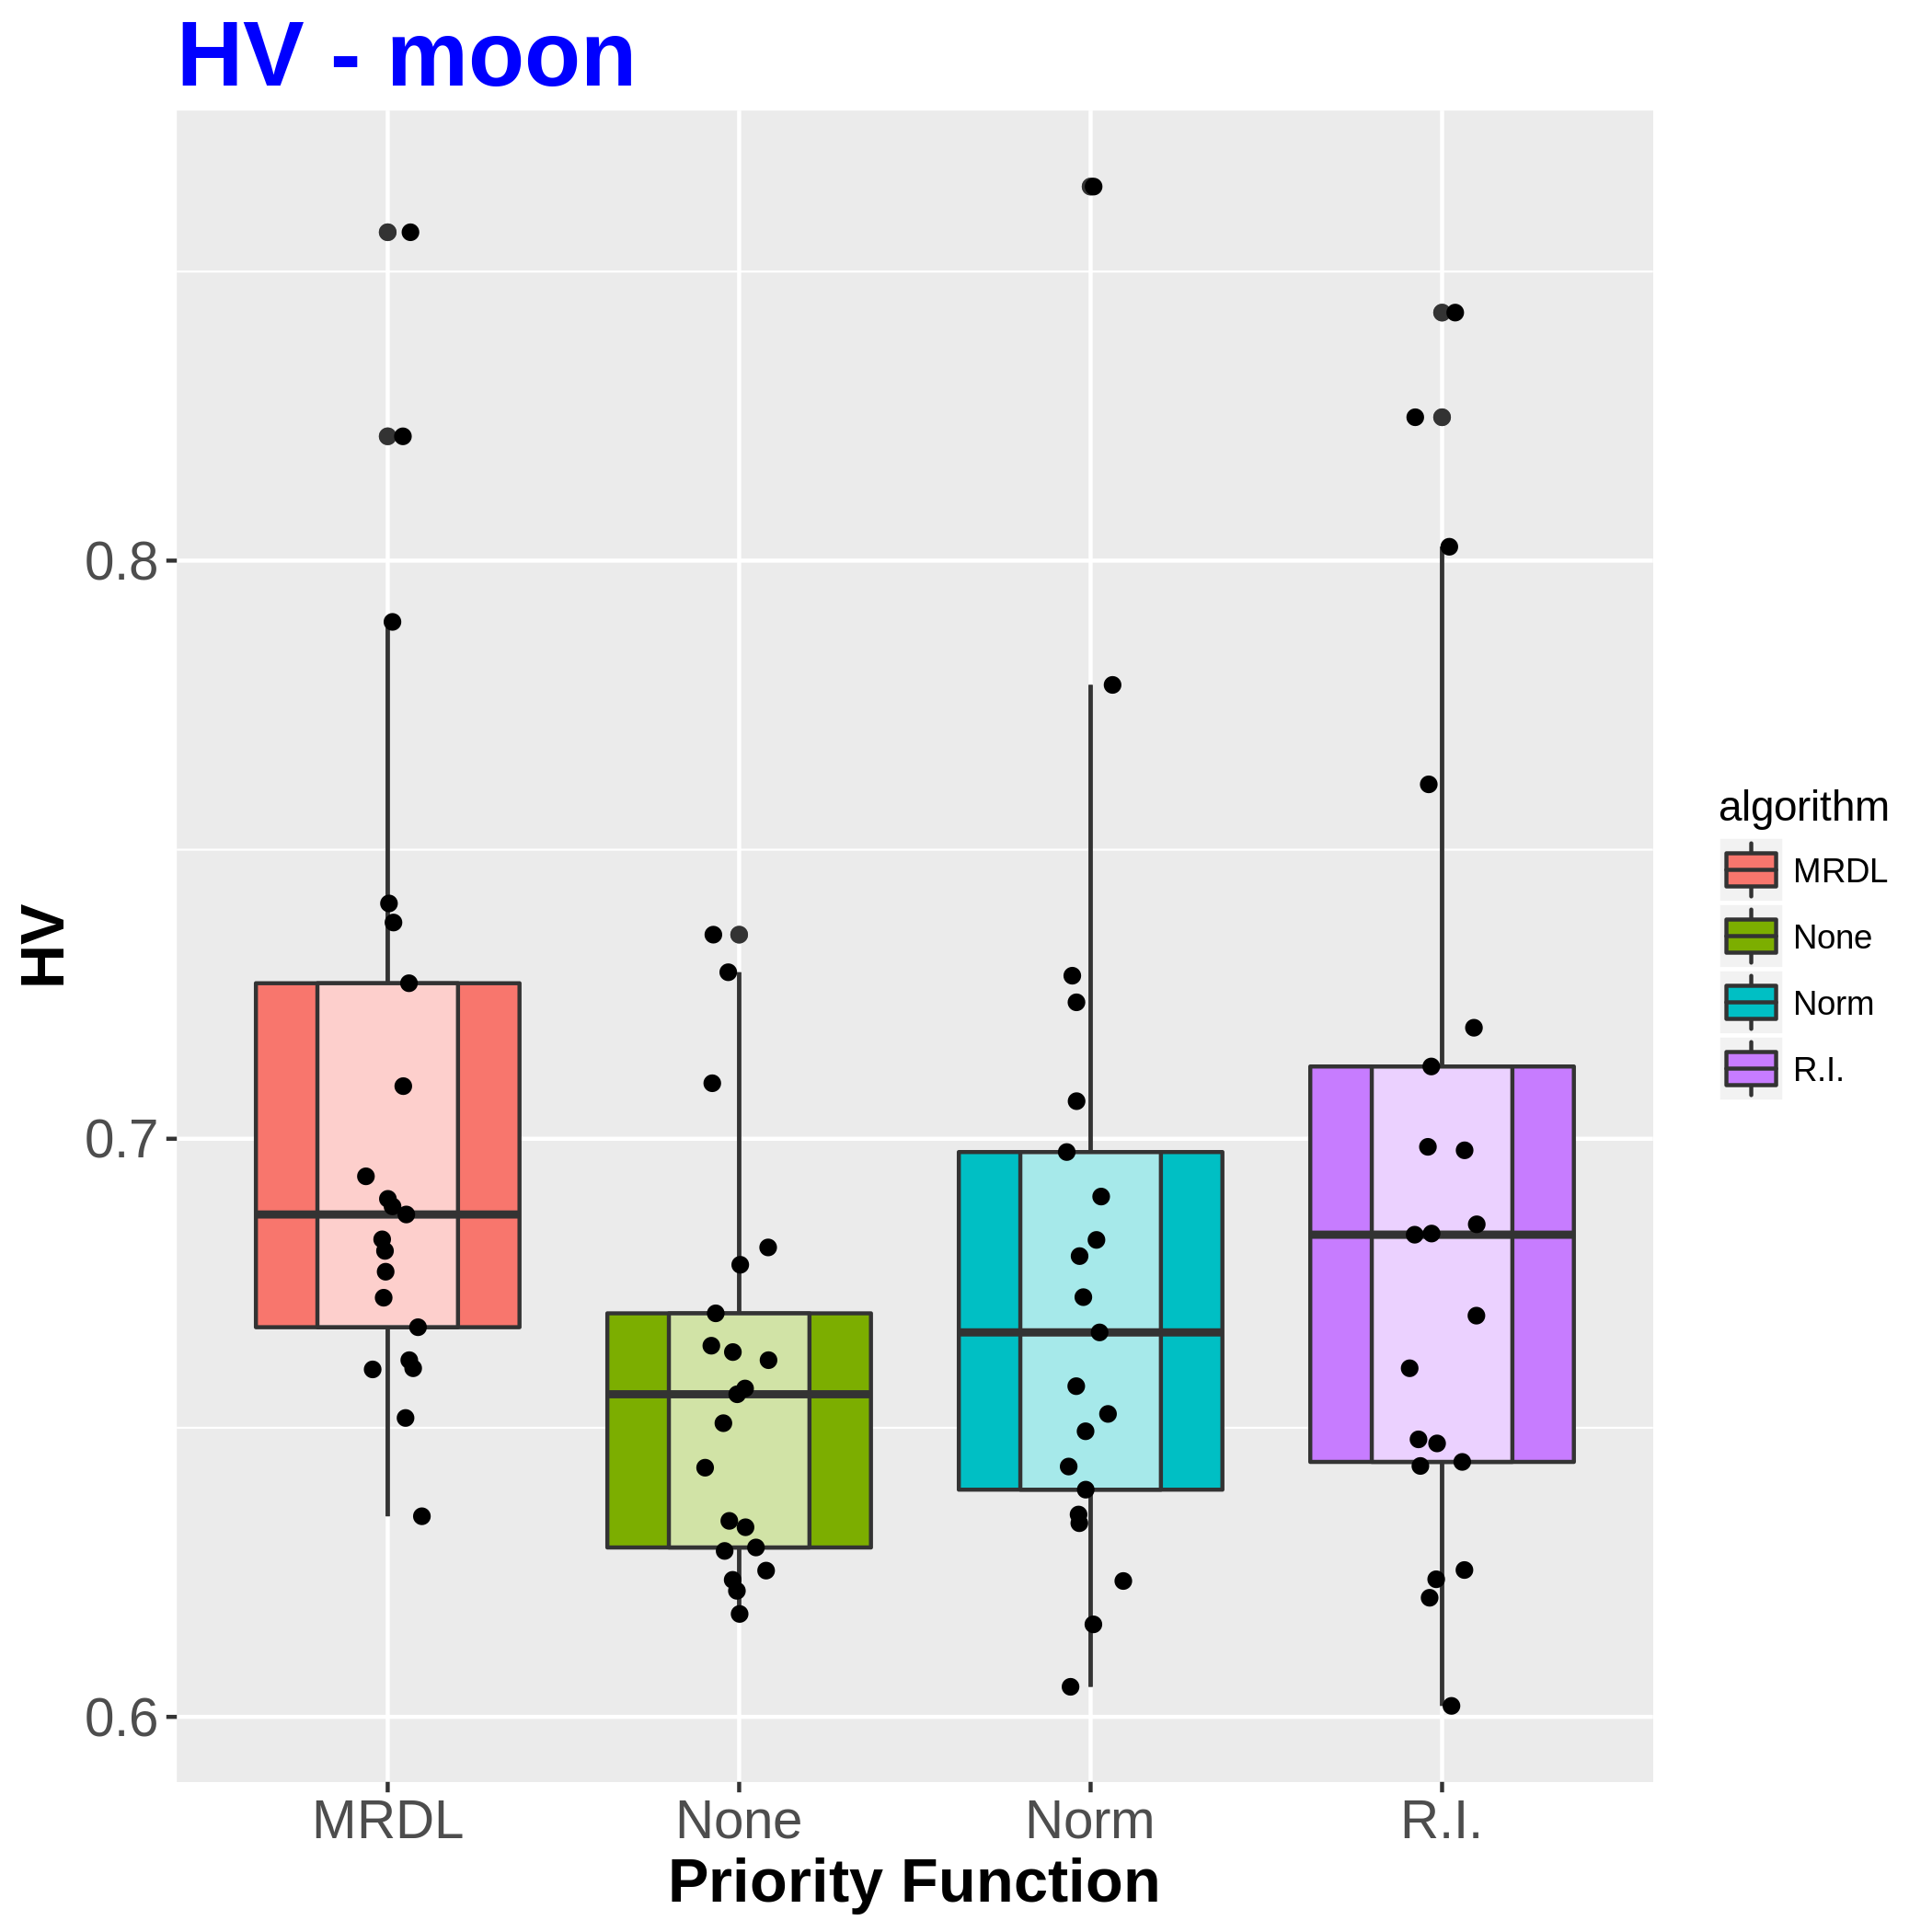
\includegraphics[width=1\textwidth, height=1\textwidth]{images/moon_HV}
%		\caption{HV values of the last iteraction on the Lunar Landing Problem}
%	\end{subfigure}
%%	\begin{subfigure}[b]{0.33\textwidth}
%%		\centering
%%		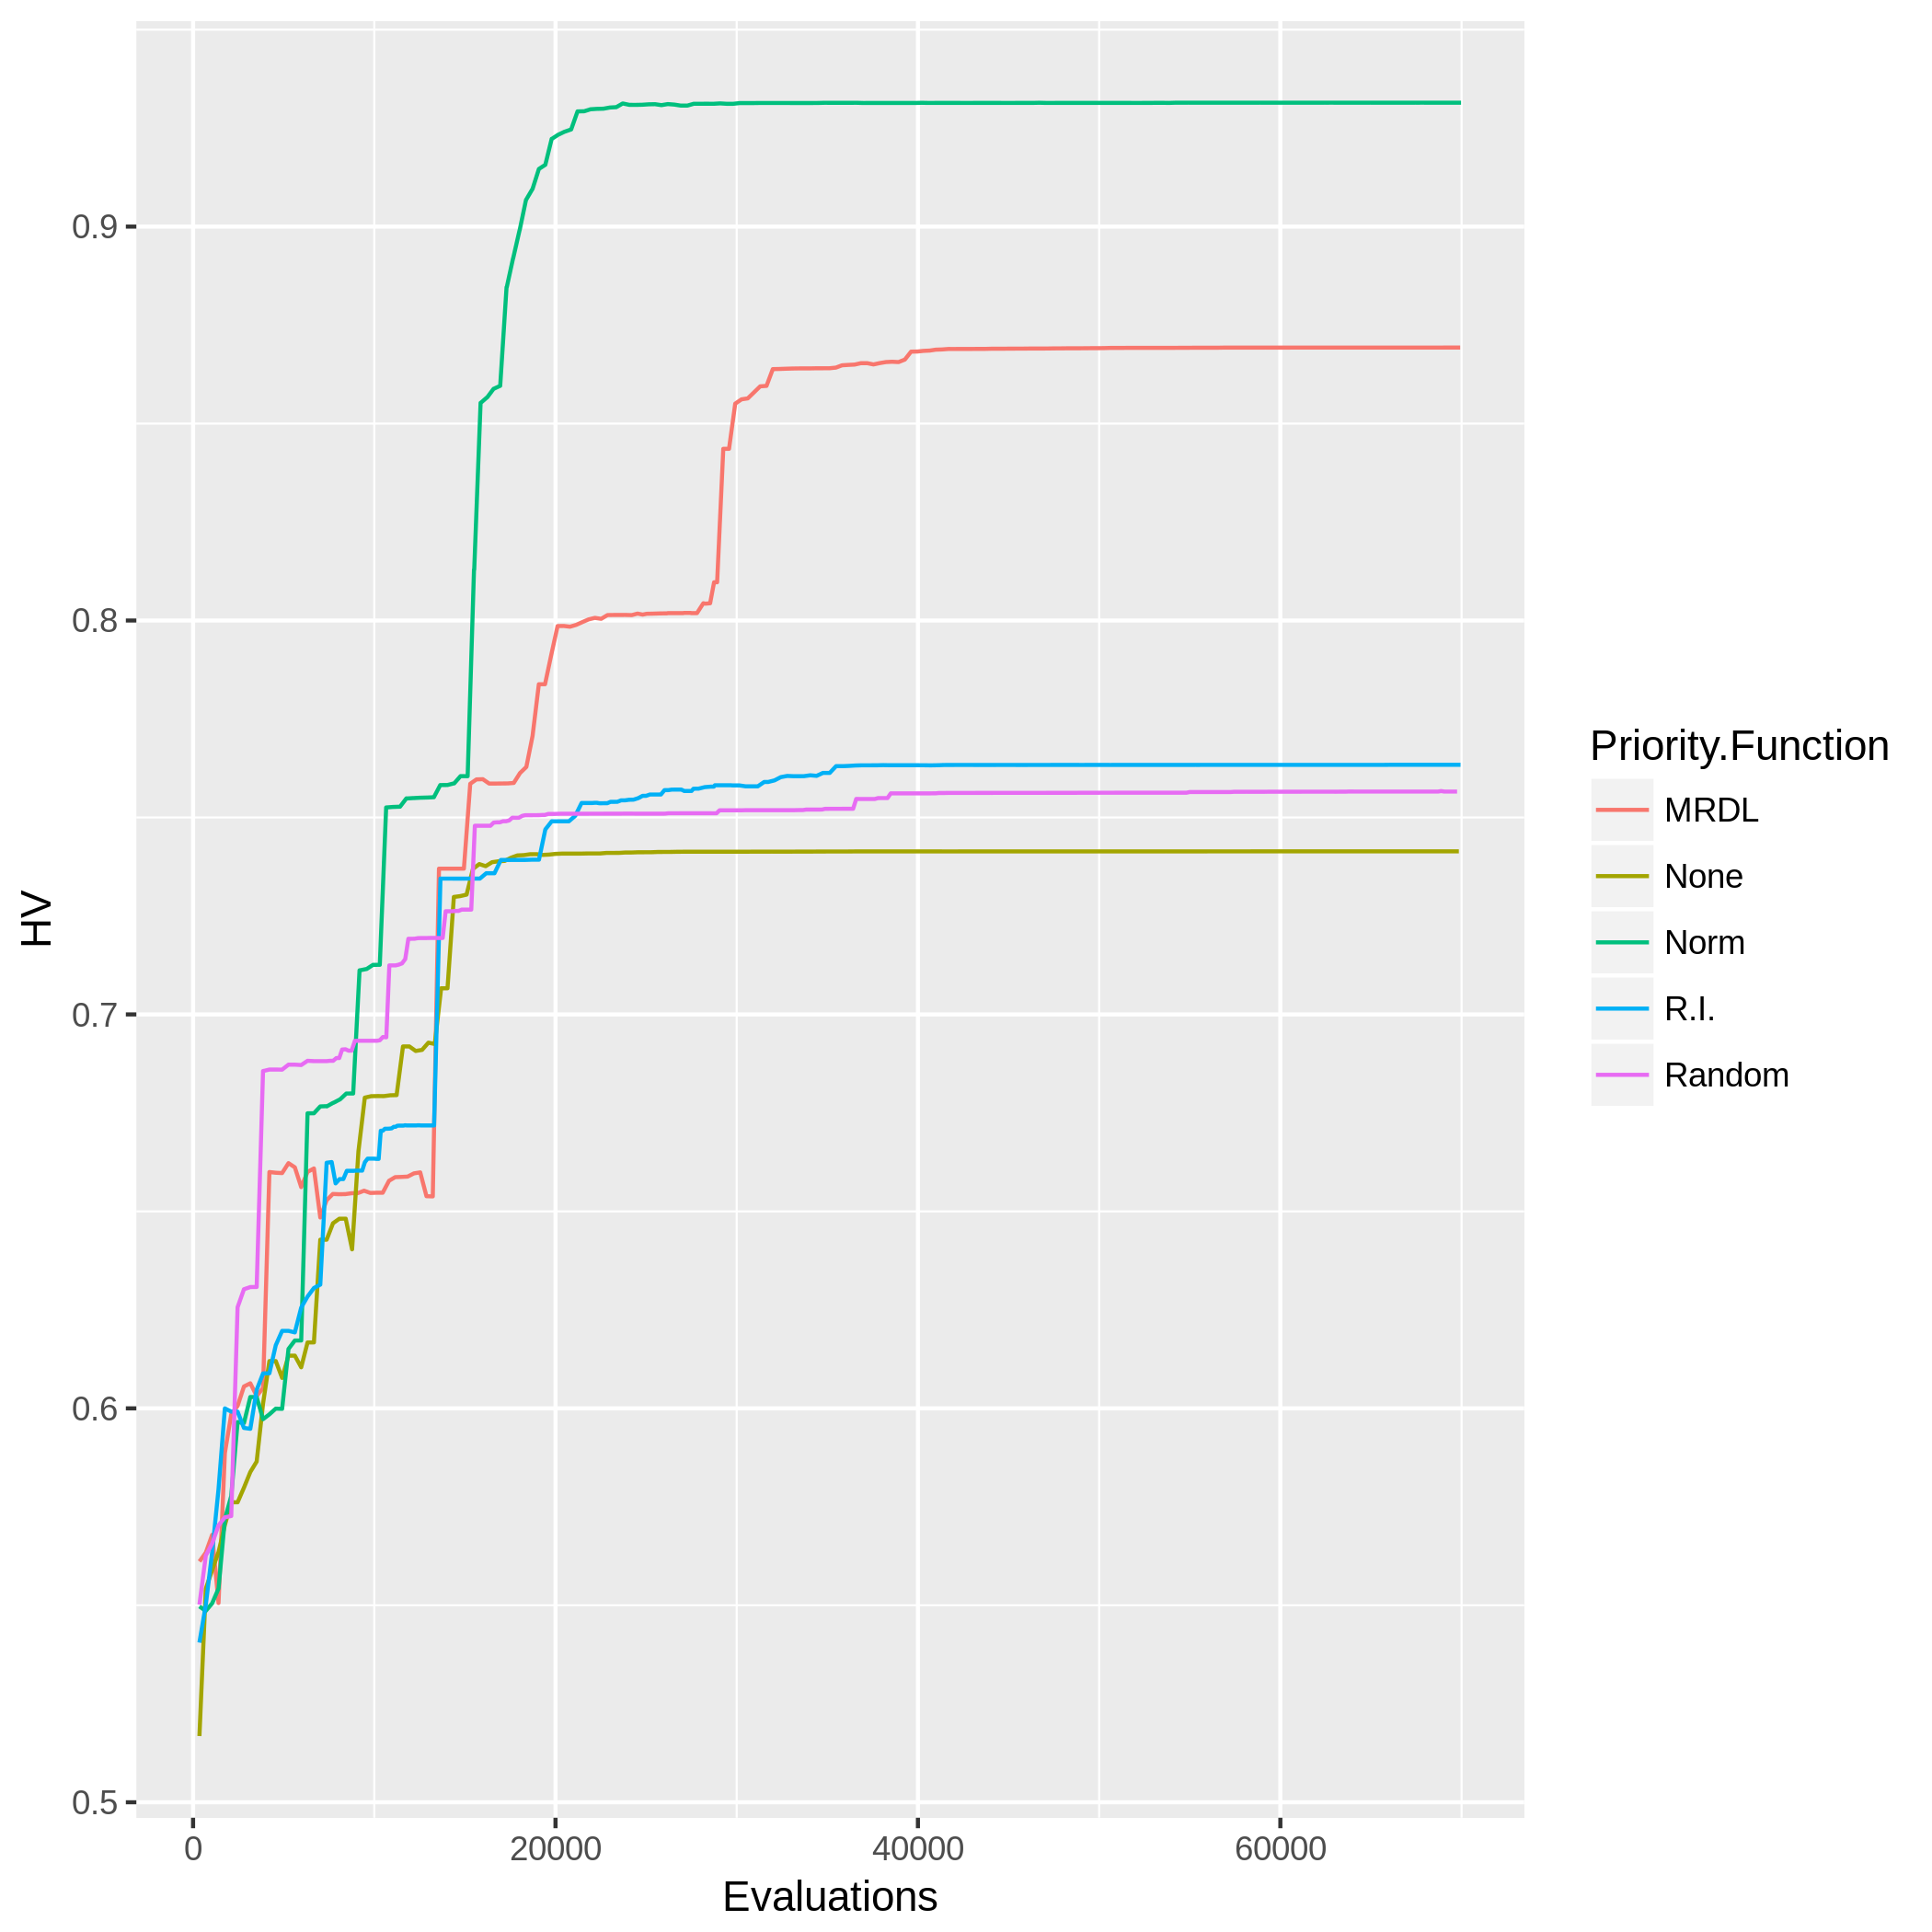
\includegraphics[width=1\textwidth, height=1\textwidth]{images/moonhv_all}
%%		\caption{Evolution of the HV on the Lunar Landing}
%%	\end{subfigure}
%	\caption{SBX crossover - ($\lambda, \lambda$) scheme.}
%	\label{moon}
%\end{figure*}



%\begin{table*}[!t]
%	\begin{tabular}{llllll}
%		\cline{6-6}
%		\hline
%		\rowcolor[gray]{.7} \multicolumn{1}{|l|}{Priority Function:}         & \multicolumn{1}{l|}{None} & \multicolumn{1}{l|}{MRDL} & \multicolumn{1}{l|}{Norm} & \multicolumn{1}{l|}{R.I.} & \multicolumn{1}{l|}{Random} \\ \hline \hline  \hline
%		\multicolumn{1}{|l|}{Lunar (Non-dominated (\%))}           & \multicolumn{1}{l}{0.69 (0.23)} & \multicolumn{1}{l}{0.87 (0.18)} & \multicolumn{1}{l}{0.83 (0.18)} & 0.69 (0.16)             &\multicolumn{1}{l|} {0.44 (0.16)} \\ \hline \hline \hline
%%		\multicolumn{1}{|l|}{Lunar (Time (seconds))}           & \multicolumn{1}{l}{32 (0.92)} & \multicolumn{1}{l}{39 (11.02)} & \multicolumn{1}{l}{46 (23.34)} & 2 (7.75)             &\multicolumn{1}{l|} {52 (0.86)} \\ \hline \hline
%		\rowcolor[gray]{.95} \multicolumn{1}{|l|}{UF1 (Non-dominated (\%))}              & \multicolumn{1}{l}{0.28 (0.03)} & \multicolumn{1}{l}{0.29 (0.05)} & \multicolumn{1}{l}{0.94 (0.10)} & 0.47 (0.09)             &\multicolumn{1}{l|} {0.68 (0.06)} \\ \hline
%%		\rowcolor[gray]{.95} \multicolumn{1}{|l|}{UF1 (Time (seconds))}              & \multicolumn{1}{l}{28 (2.36)} & \multicolumn{1}{l}{46 (2.16)} & \multicolumn{1}{l}{1 (0.60)} & 37 (3.05)            &\multicolumn{1}{l|} {34 (2.87)} \\ \hline \hline
%		\multicolumn{1}{|l|}{UF2 (Non-dominated (\%))}           & \multicolumn{1}{l}{0.34 (0.04)} & \multicolumn{1}{l}{0.34 (0.05)} & \multicolumn{1}{l}{0.96 (0.05)} & 0.61 (0.16)             &\multicolumn{1}{l|} {0.81 (0.06)} \\ \hline
%%		\multicolumn{1}{|l|}{UF2 (Time (seconds))}           & \multicolumn{1}{l}{24 (0)} & \multicolumn{1}{l}{41 (0.59)} & \multicolumn{1}{l}{1 (0.00)} & 34 (1.47)             &\multicolumn{1}{l|} {31 (0.00)} \\ \hline \hline
%		\rowcolor[gray]{.95} \multicolumn{1}{|l|}{UF3 (Non-dominated (\%))}              & \multicolumn{1}{l}{0.22 (0.03)} & \multicolumn{1}{l}{0.24 (0.03)} & \multicolumn{1}{l}{0.78 (0.13)} & 0.44 (0.15)            &\multicolumn{1}{l|} {0.59 (0.07)} \\ \hline
%%		\rowcolor[gray]{.95} \multicolumn{1}{|l|}{UF3 (Time (seconds))}              & \multicolumn{1}{l}{25 (0.22)} & \multicolumn{1}{l}{43 (1.55)} & \multicolumn{1}{l}{1 (0.60)} & 55 (2.09)           &\multicolumn{1}{l|} {31 (0.00)} \\ \hline \hline
%		\multicolumn{1}{|l|}{UF4 (Non-dominated (\%))}           & \multicolumn{1}{l}{0.58 (0.05)} & \multicolumn{1}{l}{0.60 (0.04)} & \multicolumn{1}{l}{0.90 (0.08)} & 0.75 (0.06)             &\multicolumn{1}{l|} {0.82 (0.04)} \\ \hline
%%		\multicolumn{1}{|l|}{UF4 (Time (seconds))}           & \multicolumn{1}{l}{24 (0.00)} & \multicolumn{1}{l}{41 (0.00)} & \multicolumn{1}{l}{1 (0.00)} & 34 (1.56)             &\multicolumn{1}{l|} {31 (0.22)} \\ \hline \hline
%		\rowcolor[gray]{.95} \multicolumn{1}{|l|}{UF5 (Non-dominated (\%))}              & \multicolumn{1}{l}{0.21 (0.03)} & \multicolumn{1}{l}{0.26 (0.04)} & \multicolumn{1}{l}{0.96 (0.03)} & 0.69 (0.13)             &\multicolumn{1}{l|} {0.71 (0.08)} \\ \hline
%%		\rowcolor[gray]{.95} \multicolumn{1}{|l|}{UF5 (Time (seconds))}              & \multicolumn{1}{l}{24 (0.22)} & \multicolumn{1}{l}{41 (0.60)} & \multicolumn{1}{l}{2 (0.44)} & 33 (0.54)             &\multicolumn{1}{l|} {31 (0.22)} \\ \hline \hline
%		\multicolumn{1}{|l|}{UF6 (Non-dominated (\%))}           & \multicolumn{1}{l}{0.27 (0.03)} & \multicolumn{1}{l}{0.27 (0.03)} & \multicolumn{1}{l}{0.95 (0.08)} & 0.45 (0.07)             &\multicolumn{1}{l|} {0.61 (0.07)} \\ \hline
%%		\multicolumn{1}{|l|}{UF6 (Time (seconds))}           & \multicolumn{1}{l}{24 (0.36)} & \multicolumn{1}{l}{41 (0.79)} & \multicolumn{1}{l}{1 (0.00)} & 33 (0.51)             &\multicolumn{1}{l|} {31 (0.00)} \\ \hline \hline
%		\rowcolor[gray]{.95} \multicolumn{1}{|l|}{UF7 (Non-dominated (\%))}              & \multicolumn{1}{l}{0.38 (0.06)} & \multicolumn{1}{l}{0.37 (0.05)} & \multicolumn{1}{l}{0.96 (0.03)} & 0.57 (0.11)             &\multicolumn{1}{l|} {0.80 (0.04)} \\ \hline
%%		\rowcolor[gray]{.95} \multicolumn{1}{|l|}{UF7 (Time (seconds))}              & \multicolumn{1}{l}{24 (0.30)} & \multicolumn{1}{l}{42 (0.38)} & \multicolumn{1}{l}{1 (0.46)} & 34 (0.90)             &\multicolumn{1}{l|} {31 (0.30)} \\ \hline \hline
%		\multicolumn{1}{|l|}{UF8 (Non-dominated (\%))}           & \multicolumn{1}{l}{0.40 (0.03)} & \multicolumn{1}{l}{0.39 (0.03)} & \multicolumn{1}{l}{0.70 (0.06)} & 0.67 (0.07)             &\multicolumn{1}{l|} {0.63 (0.03)} \\ \hline
%%		\multicolumn{1}{|l|}{UF8 (Time (seconds))}           & \multicolumn{1}{l}{24 (0.00)} & \multicolumn{1}{l}{39 (0.58)} & \multicolumn{1}{l}{1 (0.00)} & 51 (2.23)             &\multicolumn{1}{l|} {31 (0.30)} \\ \hline \hline
%		\rowcolor[gray]{.95} \multicolumn{1}{|l|}{UF9 (Non-dominated (\%))}              & \multicolumn{1}{l}{0.32 (0.03)} & \multicolumn{1}{l}{0.33 (0.03)} & \multicolumn{1}{l}{0.52 (0.03)} & 0.49 (0.04)             &\multicolumn{1}{l|} {0.48 (0.03)} \\ \hline
%%		\rowcolor[gray]{.95} \multicolumn{1}{|l|}{UF9 (Time (seconds))}              & \multicolumn{1}{l}{25 (0.50)} & \multicolumn{1}{l}{23 (4.59)} & \multicolumn{1}{l}{1 (27.84)} & 47 (2.75)             &\multicolumn{1}{l|} {32 (0.48)} \\ \hline \hline
%		\multicolumn{1}{|l|}{UF10 (Non-dominated (\%))}           & \multicolumn{1}{l}{0.43 (0.04)} & \multicolumn{1}{l}{0.46 (0.05)} & \multicolumn{1}{l}{0.75 (0.05)} & 0.68 (0.08)             &\multicolumn{1}{l|} {0.73 (0.06)} \\ \hline \hline \hline
%%		\multicolumn{1}{|l|}{UF10 (Time (seconds))}           & \multicolumn{1}{l}{25 (0.51)} & \multicolumn{1}{l}{38 (1.83)} & \multicolumn{1}{l}{1 (0.00)} & 47 (3.51)             &\multicolumn{1}{l|} {32 (0.30)} \\ \hline \hline
%		\rowcolor[gray]{.95} \multicolumn{1}{|l|}{DTLZ1 (Non-dominated (\%))}              & \multicolumn{1}{l}{0.05 (0.01)} & \multicolumn{1}{l}{0.07 (0.01)} & \multicolumn{1}{l}{0.98 (0.06)} & 0.62 (0.17)             &\multicolumn{1}{l|} {0.68 (0.13)} \\ \hline
%%		\rowcolor[gray]{.95} \multicolumn{1}{|l|}{DTLZ1 (Time (seconds))}              & \multicolumn{1}{l}{25 (0.90)} & \multicolumn{1}{l}{41 (1.16)} & \multicolumn{1}{l}{2 (0.00)} & 36 (10.19)             &\multicolumn{1}{l|} {32 (0.00)} \\ \hline \hline
%		\multicolumn{1}{|l|}{DTLZ2 (Non-dominated (\%))}           & \multicolumn{1}{l}{0.18 (0.03)} & \multicolumn{1}{l}{0.25 (0.03)} & \multicolumn{1}{l}{0.96 (0.05)} & 0.73 (2.93)             &\multicolumn{1}{l|} {0.84 (0.07)} \\ \hline
%%		\multicolumn{1}{|l|}{DTLZ2 (Time (seconds))}           & \multicolumn{1}{l}{25 (0.30)} & \multicolumn{1}{l}{41 (0.54)} & \multicolumn{1}{l}{1 (12.66)} & 40 (2.93)             &\multicolumn{1}{l|} {32 (0.60)} \\
%		\rowcolor[gray]{.95} \multicolumn{1}{|l|}{DTLZ3 (Non-dominated (\%))}              & \multicolumn{1}{l}{0.04 (0.02)} & \multicolumn{1}{l}{0.04 (0.02)} & \multicolumn{1}{l}{0.99 (0.05)} & 0.32 (0.17)             &\multicolumn{1}{l|} {0.44 (0.18)} \\ \hline
%%		\rowcolor[gray]{.95} \multicolumn{1}{|l|}{DTLZ3 (Time (seconds))}              & \multicolumn{1}{l}{25 (0.22)} & \multicolumn{1}{l}{40 (0.78)} & \multicolumn{1}{l}{2 (0.51)} & 32 (3.09)             &\multicolumn{1}{l|} {32 (0.22)} \\ \hline \hline
%		\multicolumn{1}{|l|}{DTLZ4 (Non-dominated (\%))}           & \multicolumn{1}{l}{0.11 (0.03)} & \multicolumn{1}{l}{0.13 (0.03)} & \multicolumn{1}{l}{0.96 (0.03)} & 0.7 (0.24)             &\multicolumn{1}{l|} {0.63 (0.13)} \\ \hline
%%		\multicolumn{1}{|l|}{DTLZ4 (Time (seconds))}           & \multicolumn{1}{l}{26 (0.36)} & \multicolumn{1}{l}{43 (1.01)} & \multicolumn{1}{l}{1 (0.00)} & 47 (5.94)             &\multicolumn{1}{l|} {33 (0.68)} \\ \hline \hline
%		\rowcolor[gray]{.95} \multicolumn{1}{|l|}{DTLZ5 (Non-dominated (\%))}              & \multicolumn{1}{l}{0.18 (0.02)} & \multicolumn{1}{l}{0.24 (0.03)} & \multicolumn{1}{l}{0.96 (0.05)} & 0.75 (0.14)             &\multicolumn{1}{l|} {0.84 (0.06)} \\ \hline
%%		\rowcolor[gray]{.95} \multicolumn{1}{|l|}{DTLZ5 (Time (seconds))}              & \multicolumn{1}{l}{2425 (1.12)} & \multicolumn{1}{l}{38 (0.49)} & \multicolumn{1}{l}{1 (0.00)} & 39 (2.83)             &\multicolumn{1}{l|} {30 (0.26)} \\ \hline \hline
%		\multicolumn{1}{|l|}{DTLZ6 (Non-dominated (\%))}           & \multicolumn{1}{l}{0.04 (0.02)} & \multicolumn{1}{l}{0.03 (0.02)} & \multicolumn{1}{l}{1.00 (0.00)} & 0.95 (0.33)             &\multicolumn{1}{l|} {0.56 (0.25)} \\ \hline
%%		\multicolumn{1}{|l|}{DTLZ6 (Time (seconds))}           & \multicolumn{1}{l}{25 (0.22)} & \multicolumn{1}{l}{38 (0.48)} & \multicolumn{1}{l}{1 (0.51)} & 33 (0.87)             &\multicolumn{1}{l|} {31 (0.30)} \\ \hline \hline
%		\rowcolor[gray]{.95} \multicolumn{1}{|l|}{DTLZ7 (Non-dominated (\%))}              & \multicolumn{1}{l}{0.13 (0.05)} & \multicolumn{1}{l}{0.13 (0.04)} & \multicolumn{1}{l}{0.97 (0.08)} & 0.66 (0.13)             &\multicolumn{1}{l|} {0.63 (0.08)} \\ \hline
%%		\rowcolor[gray]{.95} \multicolumn{1}{|l|}{DTLZ7 (Time (seconds))}              & \multicolumn{1}{l}{25 (0.22)} & \multicolumn{1}{l}{2 (0.00)} & \multicolumn{1}{l}{1 (0.00)} & 41 (1.47)             &\multicolumn{1}{l|} {30 (0.22)} \\ \hline
%	\end{tabular}
%	\caption{Percentage of the median values and the standard deviation in parenthesis of non-dominated solutions. None is the MOEA/D-DE with no priority function.}
%	\label{minor_results}
%\end{table*}

%\subsubsection{UF benchmark functions}


Figure~\ref{HVS} shows box-plot that exemplify the results found in the UF benchmark and DTLZ functions as well as the Lunar Landing problem in terms of the HV values. Figure~\ref{IGDS} does the same but in terms of the IGD values, but only to the artificial benchmarks. Finally, Figure~\ref{PFs} illustrates the PF approximation for the DTLZ4 found by all priority functions and without it. These Figures are representation of the results for other functions. The (box-plot) Figures for all functions are available in the supplementary materials.

In all these Figures, we can see that, in general, using resource allocation performs better than not using Resource Allocation. The Tables~\ref{table_hv_igd} and~\ref{minor_results} reinforces these results. The priority functions R.I., Norm, and Random achieve similar results in terms of HV values. These results are indicated by the box-plots~\ref{HVS}, the Table~\ref{table_hv_igd}, the approximation to the PF~\ref{PFs}, and the Pairwise Wilcoxon Rank Sum Tests~\ref{statistics}. We ask ourselves if the fact that Random performed as well as Norm and RI in HV indicates that there is still space for finding more appropriate priority functions. For IGD values, the same trend is confirmed, however, there is statistically significance difference between the results of Norm and R.I~\ref{statistics}. On the Lunar Landing Problem, all strategies found similar Hypervolume results (Table~\ref{table_hv_igd}). 

Now we move to the results in the Table~\ref{table_hv_igd}. It shows the results for every priority function measured by HV and IGD. In the UF functions and considering the results of the HV metric, Norm as priority function had few good results. with the best median in UF3 and UF9. The R.I. had the higher median in five functions. Surprisingly, the Random priority function got the higher median in the UF2, UF4 and UF6. When considering IGD the Norm had the best median in UF3, UF4, UF5, UF7, UF8 and UF9 functions. The R.I. had the highest median in the 4 functions. Again, Random surprised us, being the best in UF2 and UF4. In both metrics, MRDL had slightly better results than MOEA/D-DE.

Now, for the DTLZ set and first considering HV values, Norm as priority function lead to several good results in median in DTLZ2, DTLZ6 and DTLZ7 functions. R.I. performed as the best algorithm in terms of median of HV values also in 3 functions. Reinforcing our surprise, the Random priority function got the higher median in the DTLZ1, DTLZ2, DTLZ3 and DTLZ5 functions. For the values of the IGD, Norm had the best medians in the functions: DTLZ2, DTLZ5 and DTLZ6, again with the same number of best results as R.I. Here, Only in the DTLZ1 Random had the highest values.

On the Lunar Landing Problem, the best priority function in terms of median HV values is the MRDL. However, as commented above, the results are all similar. 

%That said, the best priority function in terms of median values is the MRDL.

% for the artificial benchmarks MRDL is slightly better than MOEA/D-DE, considering both HV and IGD values. Norm, R.I. and Random perform the best. On the other hand, MRDL performs the best in the Lunar problem, followed by R.I., Norm and lastly by MOEA/D-DE.


%Figure~\ref{HVS} shows box-plot that exemplify the results found in the UF benchmark and DTLZ functions as well as the Lunar Landing problem in terms of the HV values. Figure~\ref{IGDS} does the same but in terms of the IGD values, but only to the artificial benchmarks. In them we can see that for the artificial benchmarks MRDL is slightly better than MOEA/D-DE, considering both HV and IGD values. Norm, R.I. and Random perform the best. On the other hand, MRDL performs the best in the Lunar problem, followed by R.I., Norm and lastly by MOEA/D-DE.


%Figure~\ref{PFs} illustrates the PF approximation for the DTLZ4 found by all priority functions and without it. In agreement with the results given by the HV and IGD (Table~\ref{table_hv_igd}), both Norm and R.I. approximate well the PF. On the other hand it is clear that MRDL did not lead to a better approximation of the PF when compared to the one of MOEA/D-DE. More results can be found at the supplementary materials.
%
%\subsection{HV Results}
%
%Table~\ref{table_hv_igd} shows the results for every priority function measured by HV in the first part. First we discuss the results for the UF functions, then the results for the DTLZ functions and lastly the results for the Lunar Problem. Norm as priority function had few good results, with  the best median in UF3 and UF9. In UF3, there is no statistical significant difference for the R.I. while in UF9, there is no statistical significant difference for the Random. The R.I. had the higher median in five functions. Only in UF8 results there exists a statistical significant difference to the other priority functions.  In UF1, UF5 and UF7 statistical significant difference to the results of the Random. Surprisingly, the Random priority function got the higher median in the UF2 (with no statistical difference to R.I.), UF4 (with no statistical difference to R.I. or Norm) and UF6 (with no statistical difference to R.I.). MRDL had slightly better results than MOEA/D-DE, however only in UF3 and UF8 the results had statistical significance.
%
%Now, we discuss to the results on the DTLZ functions. Norm as priority function lead to several good results in median with the best median in the DTLZ2 (no statistical difference to Random), DTLZ5 (no statistical difference to Random or R.I) , DTLZ6 and DTLZ7 (no statistical difference to R.I.) cases. Only in the DTLZ6 the difference in the results had statistical significance. R.I. performed as the best algorithm in terms of median of HV values only in the DTLZ4 (without any significant difference to Random or Norm). Reinforcing our surprise, the Random priority function got the higher median in the DTLZ1 (with no statistical difference to Norm or R.I.), DTLZ2 (with no statistical difference to R.I.), DTLZ3 and DTLZ5 functions(both without statistical difference to Norm or R.I.), with its median being always higher that the one from MRDL.
%
%On the Lunar Problem, the best priority function is the MRDL, the only one with statistical difference to MOEA/D-DE. However, the results of this priority function have no statistical difference to the other priority functions.
%
%\subsection{IGD Results}
%
%We again start with the UF results and then move to the DTLZ results. In the Table~\ref{table_hv_igd} (second part) we verify that the Norm had the best median in 6 functions, being statistically different to all others in the UF3, UF5, UF7 and UF9 functions. In the UF4, the result of the Norm are not statistically different from the R.I. or the Random. In UF8 the results of the Norm not statistically different from the Random. The R.I. had the highest median in the UF1, UF4, UF6 and UF10 functions. The results of UF1 and UF4 are not statistically different from the R.I. or the Random. In UF6 the results are not statistically different from the Random while on the UF10, there is no statistical different to the results of the Norm. Norm had the best results in UF2 having the same median as Norm and R.I., with a lower standard deviation. Again, MRDL had slightly better results than MOEA/D-DE, however only in UF3 and UF8 the results had statistical significance.
%
%Moving to the DTLZ results, we verify that the Norm had the best median in 3 functions, DTLZ2, DTLZ5 (with no statistical difference to Random or R.I.) and DTLZ67 (with no statistical difference to Random). In the DTLZ2 the results had statistical difference. The R.I. perform the best in the DTLZ3 (with no statistical difference to Norm or Random), DTLZ5 and DTLZ7(both with no statistical difference to Norm). Only in the DTLZ1  Random had the highest values(with no statistical difference to Norm or R.I.).



\subsection{Proportion of Non-dominated and Feasible Solutions}

%%% Dominance and feasibility
% Another difference that we see among the Resource Allocation strategies is found in the proportion of non dominated and feasible solutions. For the Benchmark problems, the Norm Strategy achieved a very high fraction of non-dominated solutions in the final solution set. In the Lunar Landing problem, the Norm strategy achieved a higher proportion of feasible solutions than the other resource allocation strategies.It is always the fastest, mean time of the median of every function: 1.17; standard deviation (sd): 2.46. The MRDL priority function improved a little the rate of non-dominated solutions, at the cost of a longer execution time (mean time of the median of every function: 37.53; sd: 1.03). The same behavior (better rate of non-dominated solutions, more cost in time) is found in the R.I.(mean time of the median of every function: 39; sd: 5.14) and Random results (mean time of the median of every function: 31.47; sd: 0.41).

Another difference that we see among the Resource Allocation strategies is found in the proportion of non dominated and feasible solutions. The results on the Table~\ref{minor_results} indicate that the Norm strategy leads to a very high rate of non-dominated solutions in the final solution set. The MRDL priority function improved a little the rate of non-dominated solutions. The same behavior (better rate of non-dominated solutions) is found in the R.I. and Random results.

On the Lunar Landing problem, Norm had the highest rate of feasible solutions, but had the second best rate of non-dominated solutions, surpassed by R.I.


% lunar landingOn the other hand, it exceed the rate of non-dominated solutions of the MOEA/D-DE and it was the fastest, mean time of 4.95 and sd of 0.21. MOEA/D-DE had mean time of 6.67 and sd of 1.98.  Both priority functions were the slowest, Norm: mean time of 6.81 with sd of 0.40; R.I.: mean time of 6.95 and sd of 1.02.



% Figures~\ref{evolution_hv} and~\ref{evolution_igd} show how the values of the HV and IGD evolve over the iteractions of the algorithms. For the UF3 function the results caught our attention. First, it seems that more evaluations are need to a convergence of the values. Second, for the HV values the priority functions relative improvement and Norm made a "jump" over 30000 and 60000 evaluations, improving fast the HV metric values. Also at the end fo the evaluations, there is a strange regressive peak of the HV and IGD values of the Norm. That said, in most cases the values of HV and IGD converged by the end of the number evaluations (70000).

%\subsubsection{DTLZ benchmark functions}





%\subsubsection{Lunar Landing Problem}


%Figure~\ref{moon} show box-plot the results found in the Lunar Landing benchmark problem in terms of the HV values. Both priority functions related to diversity, MRDL and Norm, improved a lot the performance of the MOEA/D-DE. On the other hand, R.I. lead to a diminish of the standard deviation, with just a slight improvement on the performance. % Figure~\ref{moon} (b) show how the values of the HV evolve over the iteractions of the algorithms. All of the variants had converged around 20000 evaluations, with the exception of the MRDL (it converged with 40000). All used around half or less of the total number evaluations (70000) to converge.





\subsection{Resource Allocation}

%%% Figure 4 shows how the different strategies are allocating results for functions UF9 and DTLZ4. It is interesting to observe that RI and Norm assign similar priorities to the same subproblems in the DTLZ4. But they find opposite priorities to subproblems on the UF9 function.


Figure~\ref{RAs} illustrates the amount resource allocated by Norm, R.I. and MRDL to every subproblem on UF3 and DTLZ4 problems. We show images from the UF9 and DTLZ4 functions due to space limitations. We exclude the visuals from MOEA/D-DE since it give the same amount of resource to every problem (200) and of the Random, since it is uniformly noisy.

It is clear from this Figure~\ref{RAs} that, during the execution of the algorithm, the Resource Allocation to each subproblem is different. This behavior is also different for each priority functions, illustrating that every priority function allocates different amount of resource given their characteristics. It is also important to highlight that each priority function influences the search differently given different MOPs.

We highlight that the results form the priority functions Norm and R.I. in the UF9 function, since it appears to be that they prioritized subproblems in an opposite way. In the DTLZ4 they appear to prioritize similar subproblems, assigning similar priorities to the same subproblems. The distribution of resources is less abrupt in the case of Norm, however R.I. had better results, in these problems. MRDL influences weakly the distribution of Resource Allocation, which might indicate its poor performance. In both MRDL cases shown the distribution got closer to 200 resources per subproblem, similar to not using any priority function.





%\subsubsection{Non-Dominated Solutions and Execution Time}
